

%\todo[inline]{I suggest to start the results section a bit broader, instead of diving into details right away. }

This chapter will present the results of the binary and linear BPCRR models, with respect to predictive performance and agreement between the models. The results are divided into simulation and application results, respectively. We start be presenting the simulation results, where we look at, predictive performance on the observation scale, correctness of the estimated breeding values, and the models ability to recover the true amount of additive genetic variance. Next, we apply the binary and linear BPCRR to data from the Helgeland study system, we start by selecting the number of PCs to use, and then compare the models predictive performance with the standard model in the field. Then, we look at the agreement between the predictions and the estimated breeding values from the linear and binary BPCRR models. The results presented establish the basis for the discussion in the next chapter. 

 

\section{Simulation results}

% ------------------ 1) AUC results ------------------

For the simulations we have looked at the PR-AUC for predictive performance on the observation scale, Spearman correlation between the true breeding values and the estimated breeding values, and lastly the amount of the true additive genetic variance the models managed to reconstruct, as a function of the number of PCs included in the model. All results will be summarized over $10$ replicates and we simulated two different responses. 

Overall, the PR-AUC patterns differed across heritability levels. Higher heritability led to higher PR-AUC values, whereas accuracy remained relatively stable across most values of $K$ (\autoref{fig:bin_auc_vs_K_h2_whole}, \autoref{fig:lin_auc_vs_K_h2}). In addition, there were no substantial differences between the binary and linear models.
%
When interpreting PR-AUC, it should be compared with the prevalence in the dataset, which in this case is $0.5$ by construction. For $h^2 = 0.1$, the binary model shows fairly stable PR-AUC values across the full range of $K$, around $0.54$--$0.57$, in both simulation settings. The PR-AUC of the linear model closely follows that of the binary model (\autoref{fig:lin_auc_vs_K_h2}). There is no clear pattern of either increasing or decreasing PR-AUC as a function of $K$. In relative terms, both models perform approximately $8$--$14\%$ better than a random classifier, for which the expected PR-AUC is $0.5$.
%
For $h^2 = 0.2$, we observe a slight increase in PR-AUC for all $K$ compared with $h^2 = 0.1$. There also appears to be an increase in PR-AUC at lower values of $K$, from $K = 100$ to $K = 500$, after which it stabilizes around $0.57$. The same pattern is visible for the linear model. This corresponds to an approximately $14\%$ relative improvement in predictive performance on the observation scale for both models.
%
Increasing $h^2$ further to $0.33$ improves accuracy in both models to around $0.62$, corresponding to a $24\%$ relative improvement compared with a random classifier. The PR-AUC also increases up to $K = 500$, and more rapidly than for $h^2 = 0.2$, rising from $0.58$ to a peak of $0.63$ before stabilizing at higher values of $K$. 
\\

% ---------------------- AUC figures -----------------------
\todo[inline]{General comment regarding figures: make labels readable. This holds also for titles and scales along the axes. Also, make titles short and clear. In 4.1.1, the title could be "Binary models, simulations" and in 4.1.2 "Linear models, simulations". The fact that this is PR-AUC is visible from the y-axis label, and the fact that these are PCs is visible from the x-axis labels. Only give the information that is needed and lacking.}
% AUC figure BINARY
\begin{figure}[htbp]
    \centering
    \begin{subfigure}[b]{\textwidth}
        \centering
        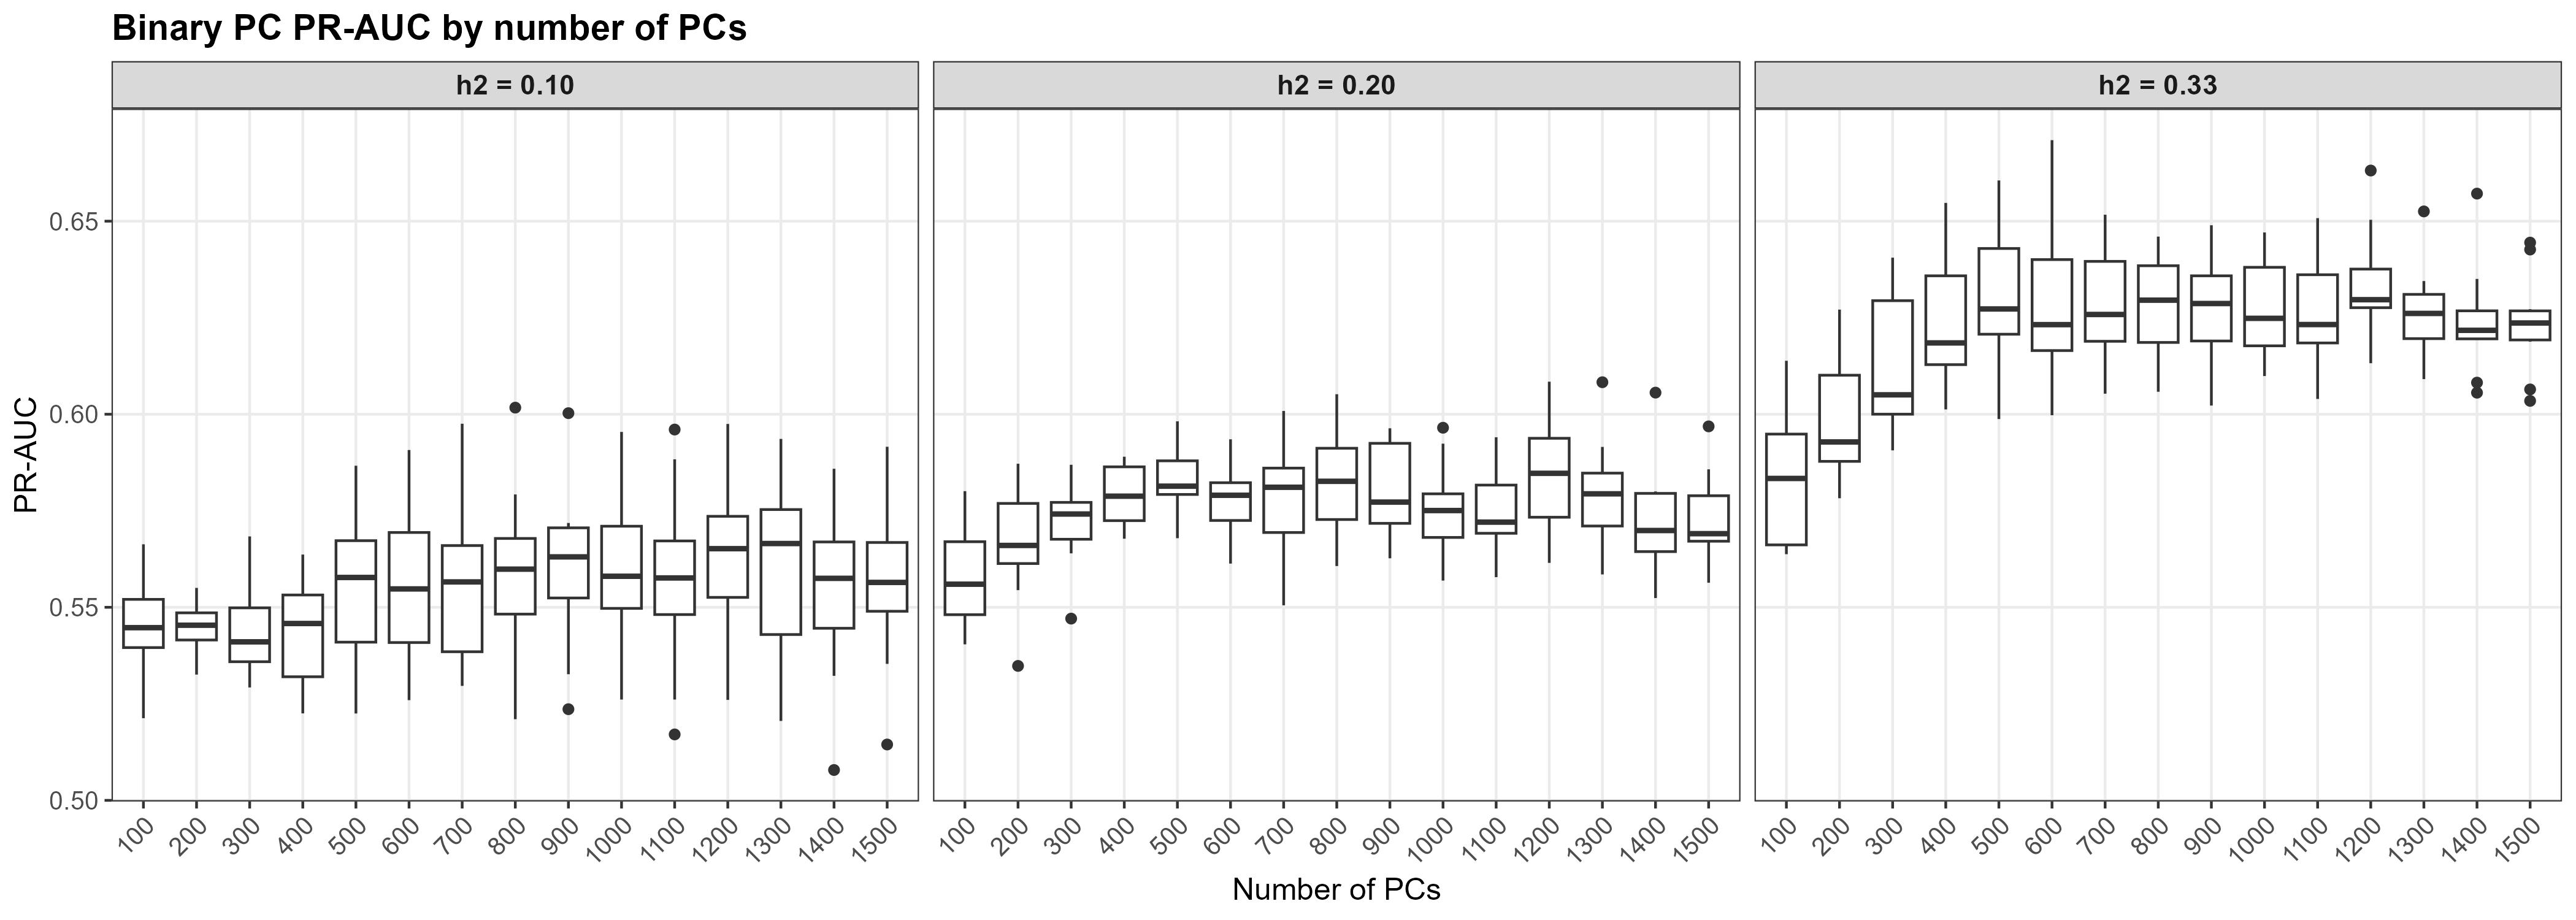
\includegraphics[width=\textwidth]{Figures/Results/simulations/bin_pr_auc_vs_pc_combined.jpg}
    \end{subfigure}

    \vspace{0.5cm}

    \begin{subfigure}[b]{\textwidth}
        \centering
        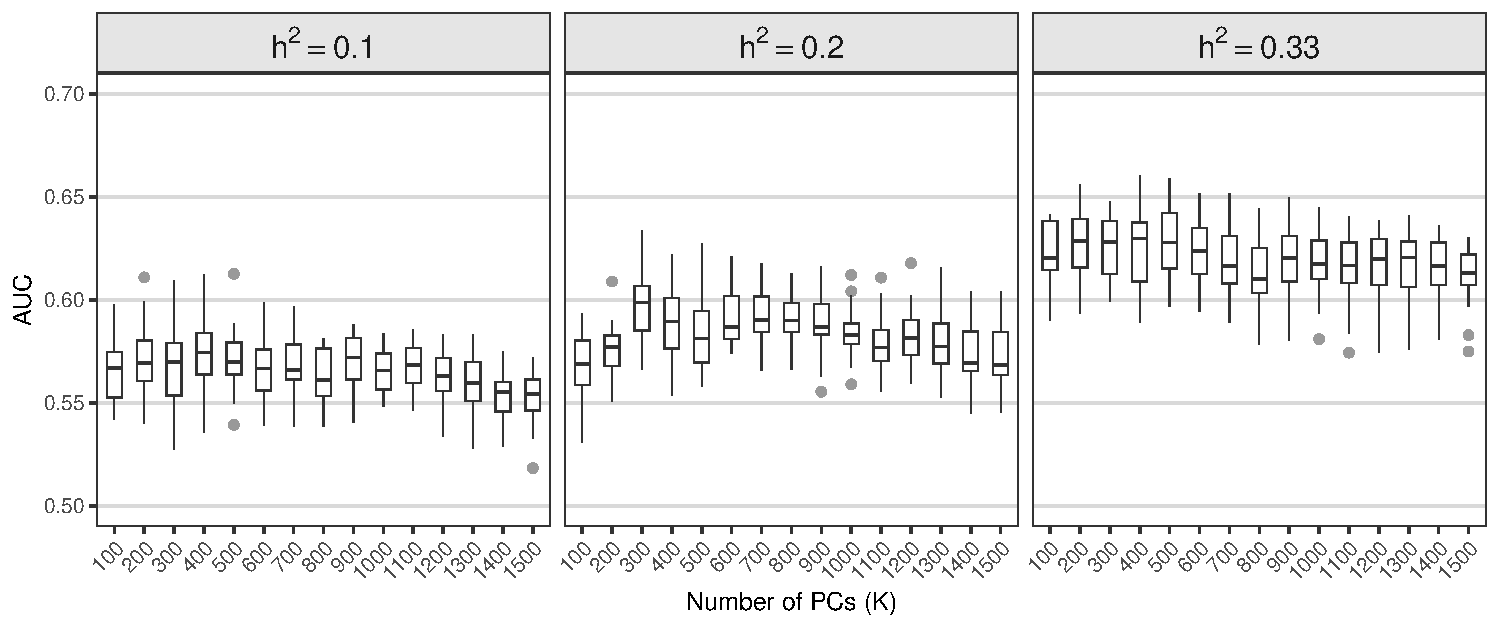
\includegraphics[width=\textwidth]{Figures/Results/simulations/auc_vs_K_h2_grid.pdf}
    \end{subfigure}
    \caption[
    Classification accuracy of the binary model on the observed scale.
    ]{
     PLACEHOLDER FOR NEW BINARY SIM FIG. PR-AUC of the binary model as a function of the number of principal components ($K$) for three heritability levels.
    Boxplots show the distribution across 10 independent replicates, with the horizontal line indicating the median PR-AUC.  For the three heritability levels $h^2 = 0.1$, $0.2$, and $0.33$, the reference PR-AUC values were $0.64$, $0.71$, and $0.78$, respectively.
    }
    \label{fig:bin_auc_vs_K_h2_whole}
\end{figure}


% AUC figure LINEAR
\begin{figure}[htbp]
    \centering
    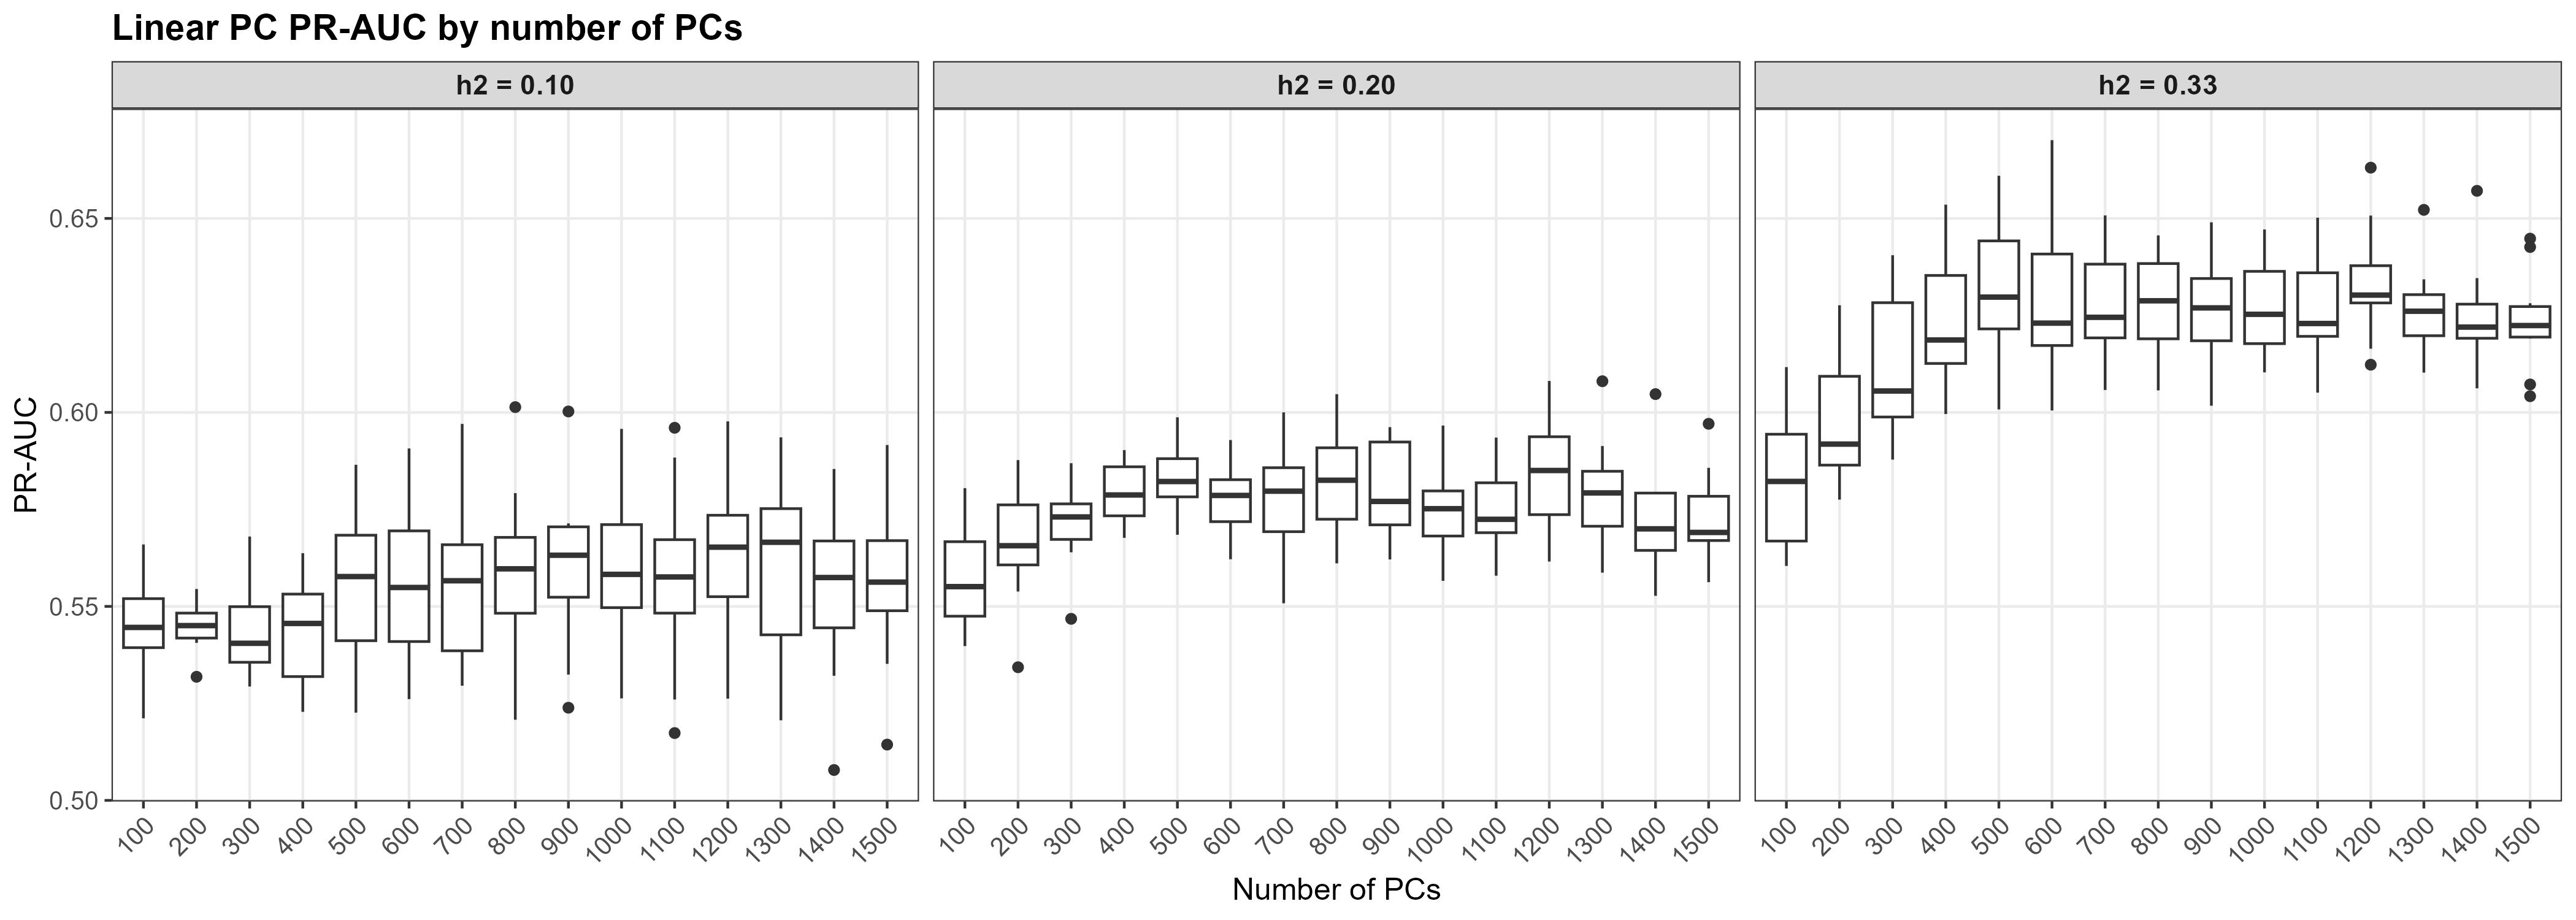
\includegraphics[width=\textwidth]{Figures/Results/simulations/pr_auc_vs_pc_combined.jpg}
    \caption[
    Classification accuracy of the linear model on the observed scale.
    ]{
    PLACEHOLDER FOR NEW LINEAR SIM FIG. PR-AUC of the linear model as a function of the number of principal components ($K$) for three heritability levels.
    Boxplots show the distribution across 10 independent replicates, with the horizontal line indicating the median PR-AUC.
    }
    \label{fig:lin_auc_vs_K_h2}
\end{figure}

% ------------------- Correlation results ------------------

Overall, the correlation patterns differed across heritability levels, but were quite similar between the linear and binary models (\autoref{fig:bin_corr_vs_K_h2_whole}, \autoref{fig:lin_corr_vs_K_h2}). Higher heritability was associated with higher correlations. For all three heritability levels, the maximal median correlation appeared at moderate values of $K$, around $400$--$600$. The linear model closely followed the binary model. In addition, there was a peak in correlation as a function of $K$.
%
For $h^2 = 0.1$, the Spearman correlation with the true breeding values showed very similar patterns for the two models. The correlation increased to a maximal median at $K = 500$, and then decreased slightly. The difference between the highest and lowest median correlation across all values of $K$ was quite small, with an absolute range of $0.044$ for both models.
%
For $h^2 = 0.2$, the overall correlation was higher for all values of $K$ than for $h^2 = 0.1$, again with a maximal correlation at $K = 500$ for both models. The median correlation ranged from $0.30$ to $0.37$, and the same decline after the peak was observed.
%
For $h^2 = 0.33$, the overall level of correlation increased further compared with $h^2 = 0.2$. We also observed a steeper increase from $K = 100$ to $K = 500$, and a larger overall range, with the correlation varying from $0.32$ to $0.45$. 

% include plots/results on which K for the Aspheim theory that should give maximal correlation. 

% --------------------- Correlation figures ------------------

% correlation figure BINARY
\begin{figure}[htbp]
    \centering
    \begin{subfigure}[b]{\textwidth}
        \centering
        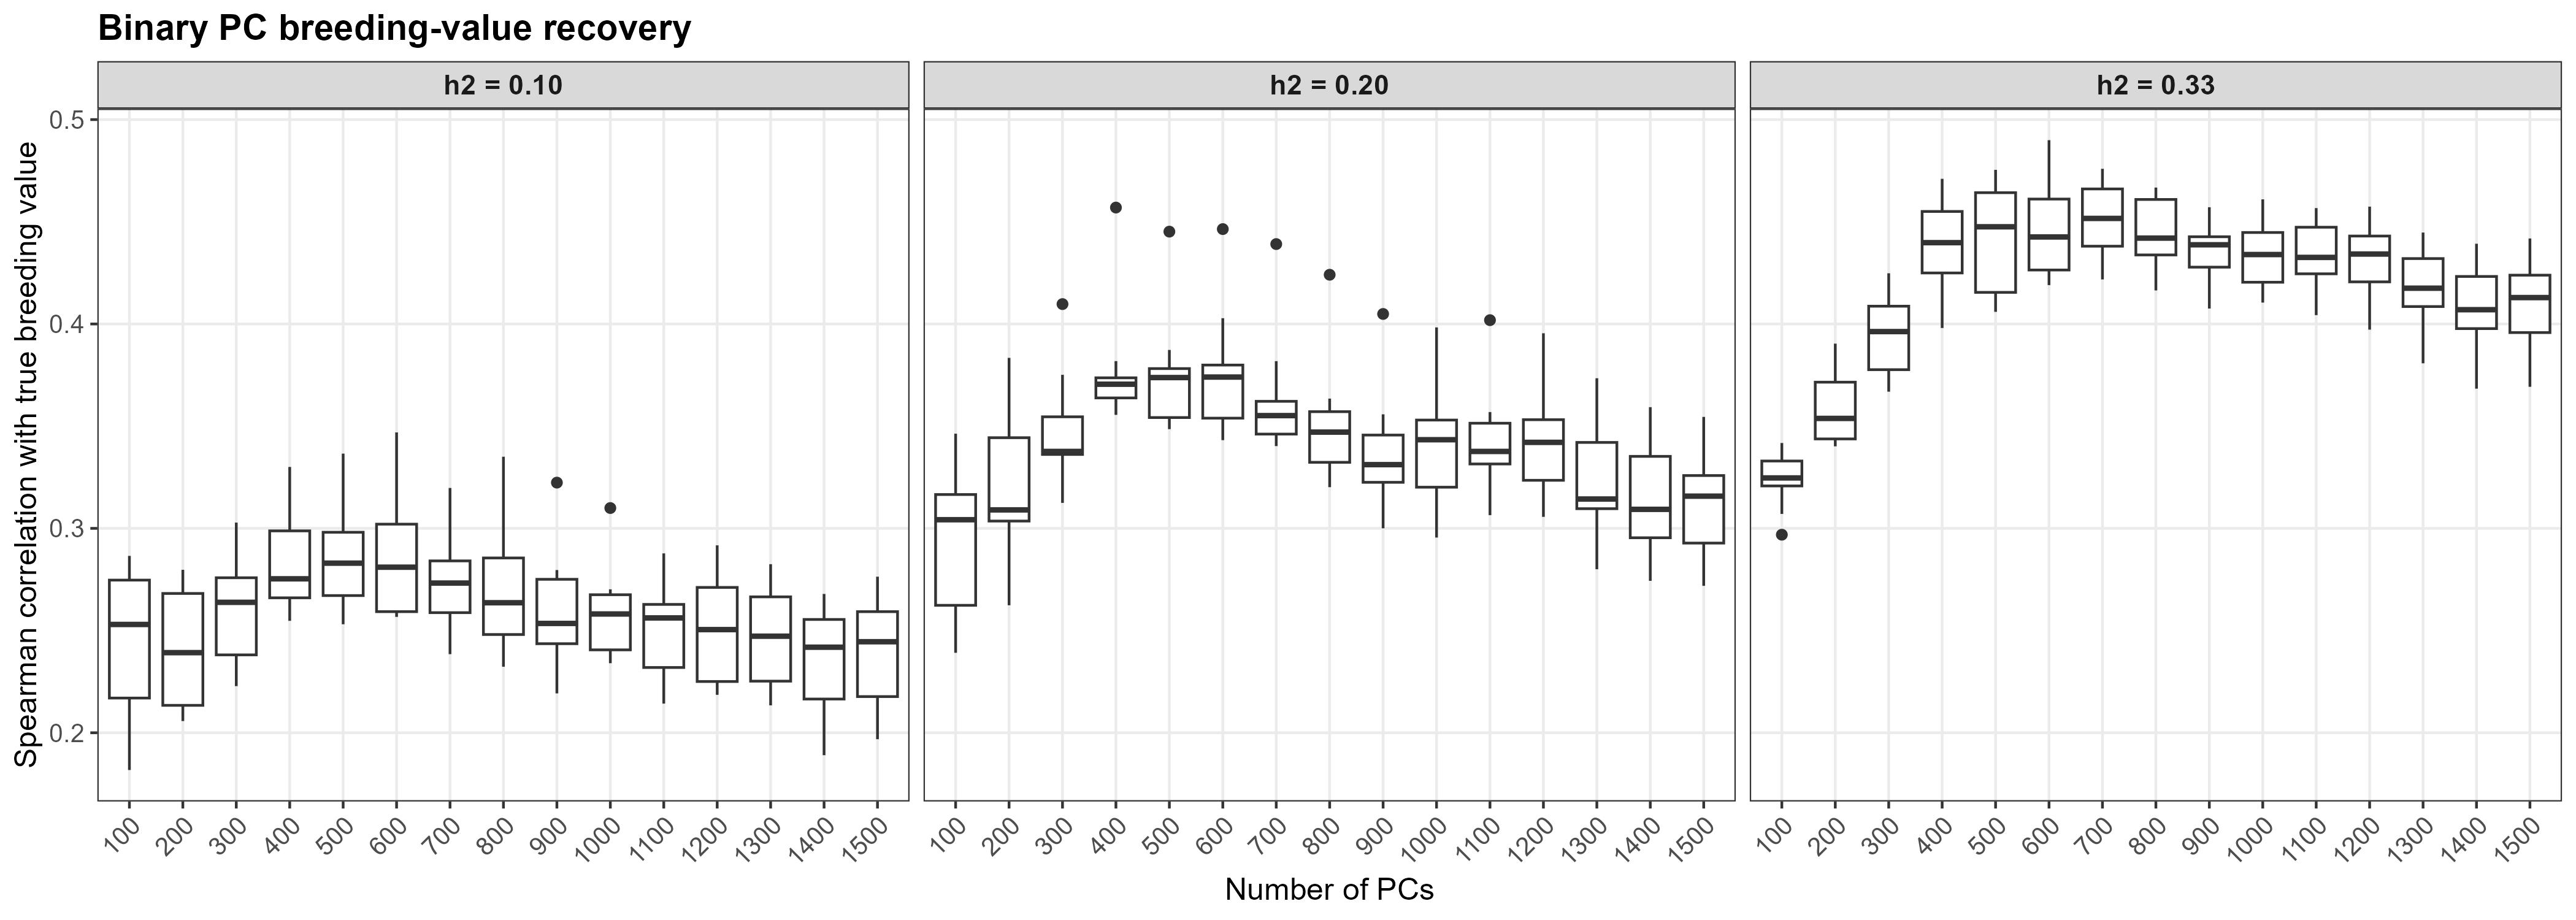
\includegraphics[width=\textwidth]{Figures/Results/simulations/bin_correlation_vs_pc_combined.jpg}
        \label{fig:bin_corr_vs_K_h2_master}
    \end{subfigure}

    \vspace{0.5cm}

    \begin{subfigure}[b]{\textwidth}
        \centering
        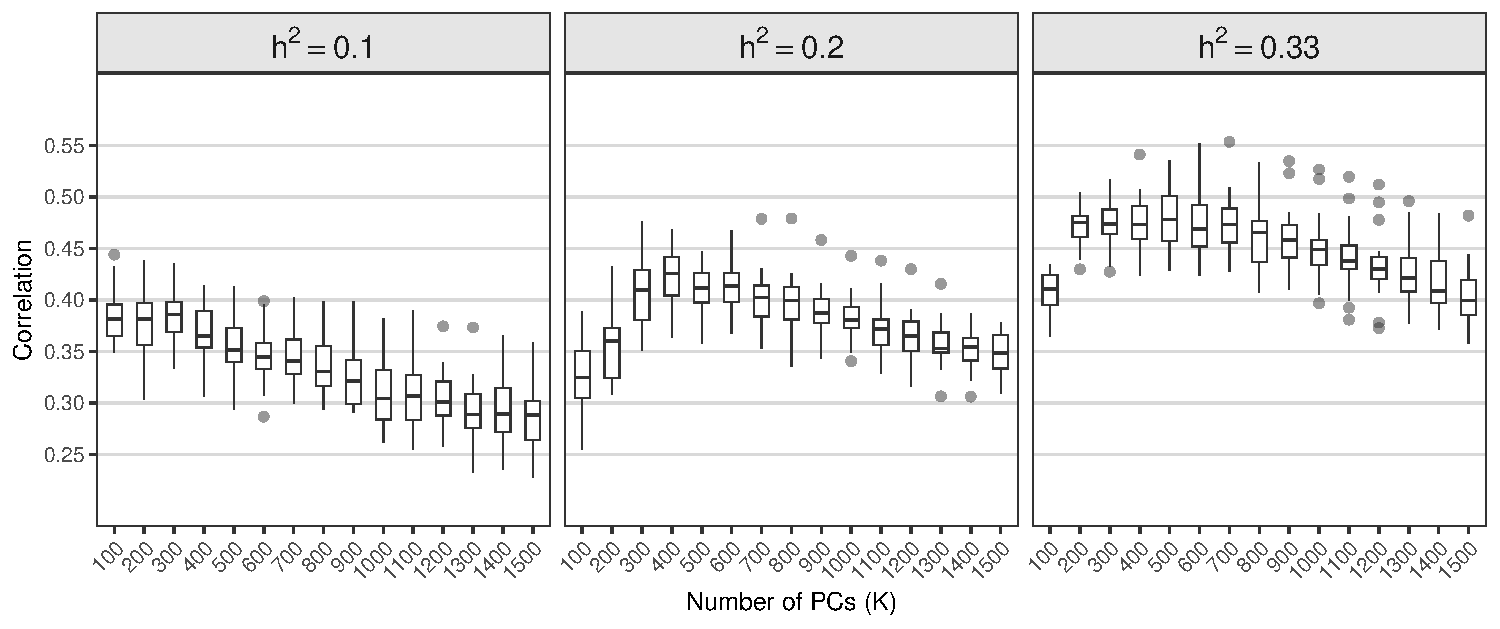
\includegraphics[width=\textwidth]{Figures/Results/simulations/corr_vs_K_h2_grid.pdf}
        \label{fig:bin_corr_vs_K_h2_project}
    \end{subfigure}
    \caption[
    Classification accuracy of the linear model on the latent scale
    ]{
    Correlation between the true and the predicted breeding values for the binary model as a function of the number of principal components ($K$) for three heritability levels.
    Boxplots show the distribution across 10 independent replicates, with the horizontal line indicating the median correlation.
    }
    \label{fig:bin_corr_vs_K_h2_whole}
\end{figure}

% Correlation figure LINEAR
\begin{figure}[htbp]
    \centering
    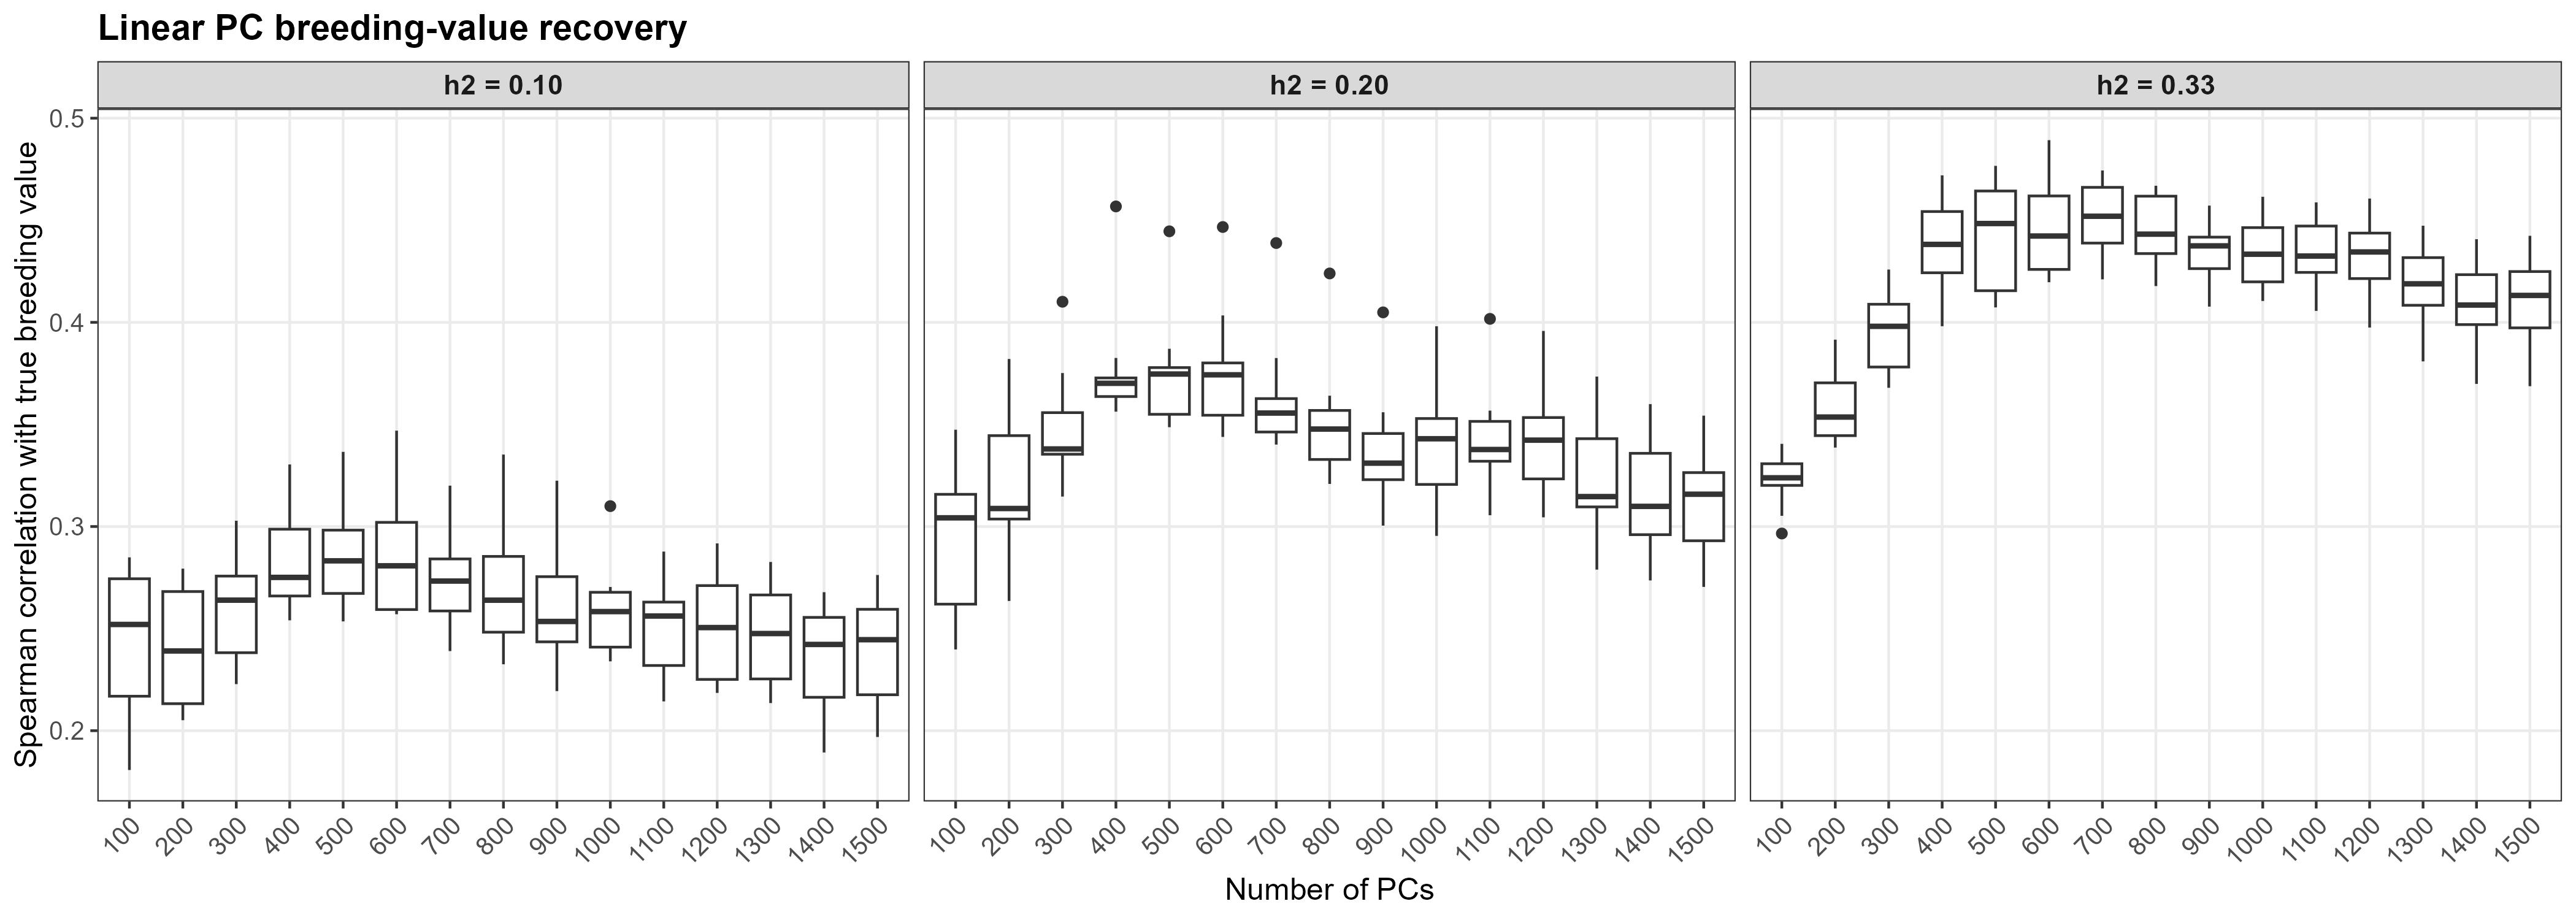
\includegraphics[width=\textwidth]{Figures/Results/simulations/correlation_vs_pc_combined.jpg}
    \caption[
    Correlation of the linear model on the observed scale
    ]{
    correlation of the linear model as a function of the number of principal components ($K$) for three heritability levels.
    Boxplots show the distribution across 10 independent replicates, with the horizontal line indicating the median correlation.
    }

    \label{fig:lin_corr_vs_K_h2}
\end{figure}

% --------------------- Heritability results ---------------

Overall, both the binary and the linear model reconstructed the additive genetic variance, quite well (\autoref{fig:h2_vs_K_combined}). Across all heritability scenarios, the proportion of reconstructed additive genetic variance increased as the number of principal components $K$ grew, although the rate of increase differed noticeably between scenarios. When heritability was low, a substantial share of the variance was captured by the first $100$ components, whereas for higher heritabilities the increase was more gradual and did not reach the same level of recovery within the examined range of $K$.
%
For $h^2 = 0.1$, the first $100$ PCs reconstructed $51\%$ of the total latent additive genetic variance in the binary model and $50\%$ of the total observed-scale additive genetic variance in the linear model. At $K = 300$, both models had reconstructed almost $80\%$ of the true total additive genetic variance on their respective scales. Beyond this point, the gains from adding more PCs became smaller, and by $K = 1500$ essentially all heritability was reconstructed.
%
For $h^2 = 0.2$, the first $100$ PCs reconstructed $35\%$ of the total latent additive genetic variance in the binary model, while the linear model reconstructed $37\%$ of the total observed-scale additive genetic variance. To recover $80\%$ of the additive genetic variance, around $500$ PCs were needed. We also observed that at $K = 1500$, the recovered additive genetic variance was still not as close to the true value as in the case $h^2 = 0.1$.
%
For $h^2 = 0.33$, the first $100$ PCs reconstructed $33\%$ of the total latent additive genetic variance in the binary model and $32\%$ of the total observed-scale additive genetic variance in the linear model. To recover $80\%$ of the total additive genetic variance, $600$ PCs were needed for the binary model and $700$ PCs for the linear model. We also see that in both cases the reconstructed additive genetic variance remained further from the true value than in the lower-heritability scenarios. 

% -------------------- Heritability figures ----------------

% Heritability figure BINARY
\begin{figure}[htbp]
    \centering

    \begin{subfigure}[t]{\textwidth}
        \centering
        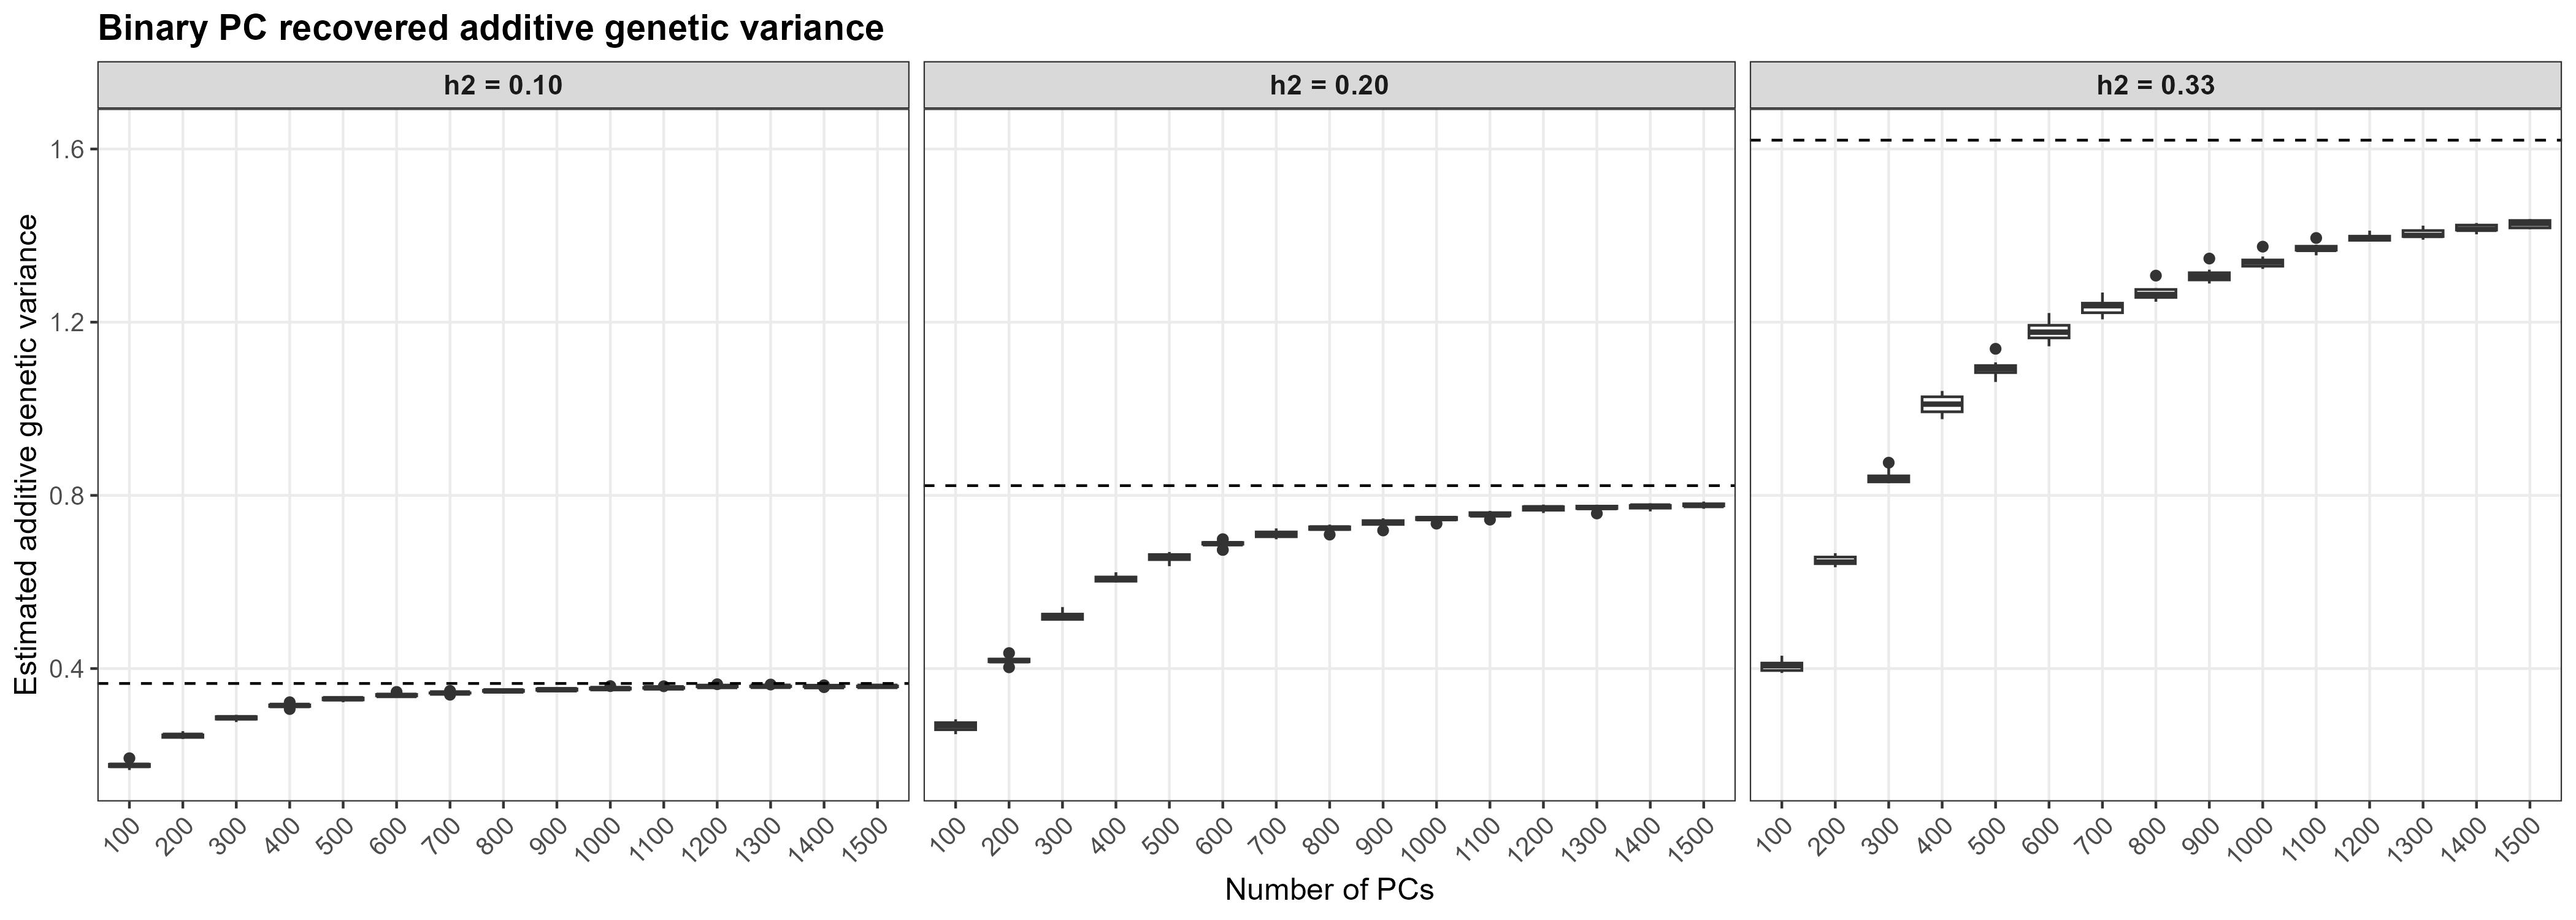
\includegraphics[width=\textwidth]{Figures/Results/simulations/bin_additive_genetic_variance_vs_pc_combined.jpg}
        \caption{Recovered heritability by the binary model as a function of the number of principal components ($K$) for three heritability levels. Boxplots show the distribution across 10 independent replicates, and the horizontal line shows the true observation-scale heritability in each scenario.}
        \label{fig:bin_h2_vs_K_h2}
    \end{subfigure}

    \vspace{0.5cm}

    \begin{subfigure}[t]{\textwidth}
        \centering
        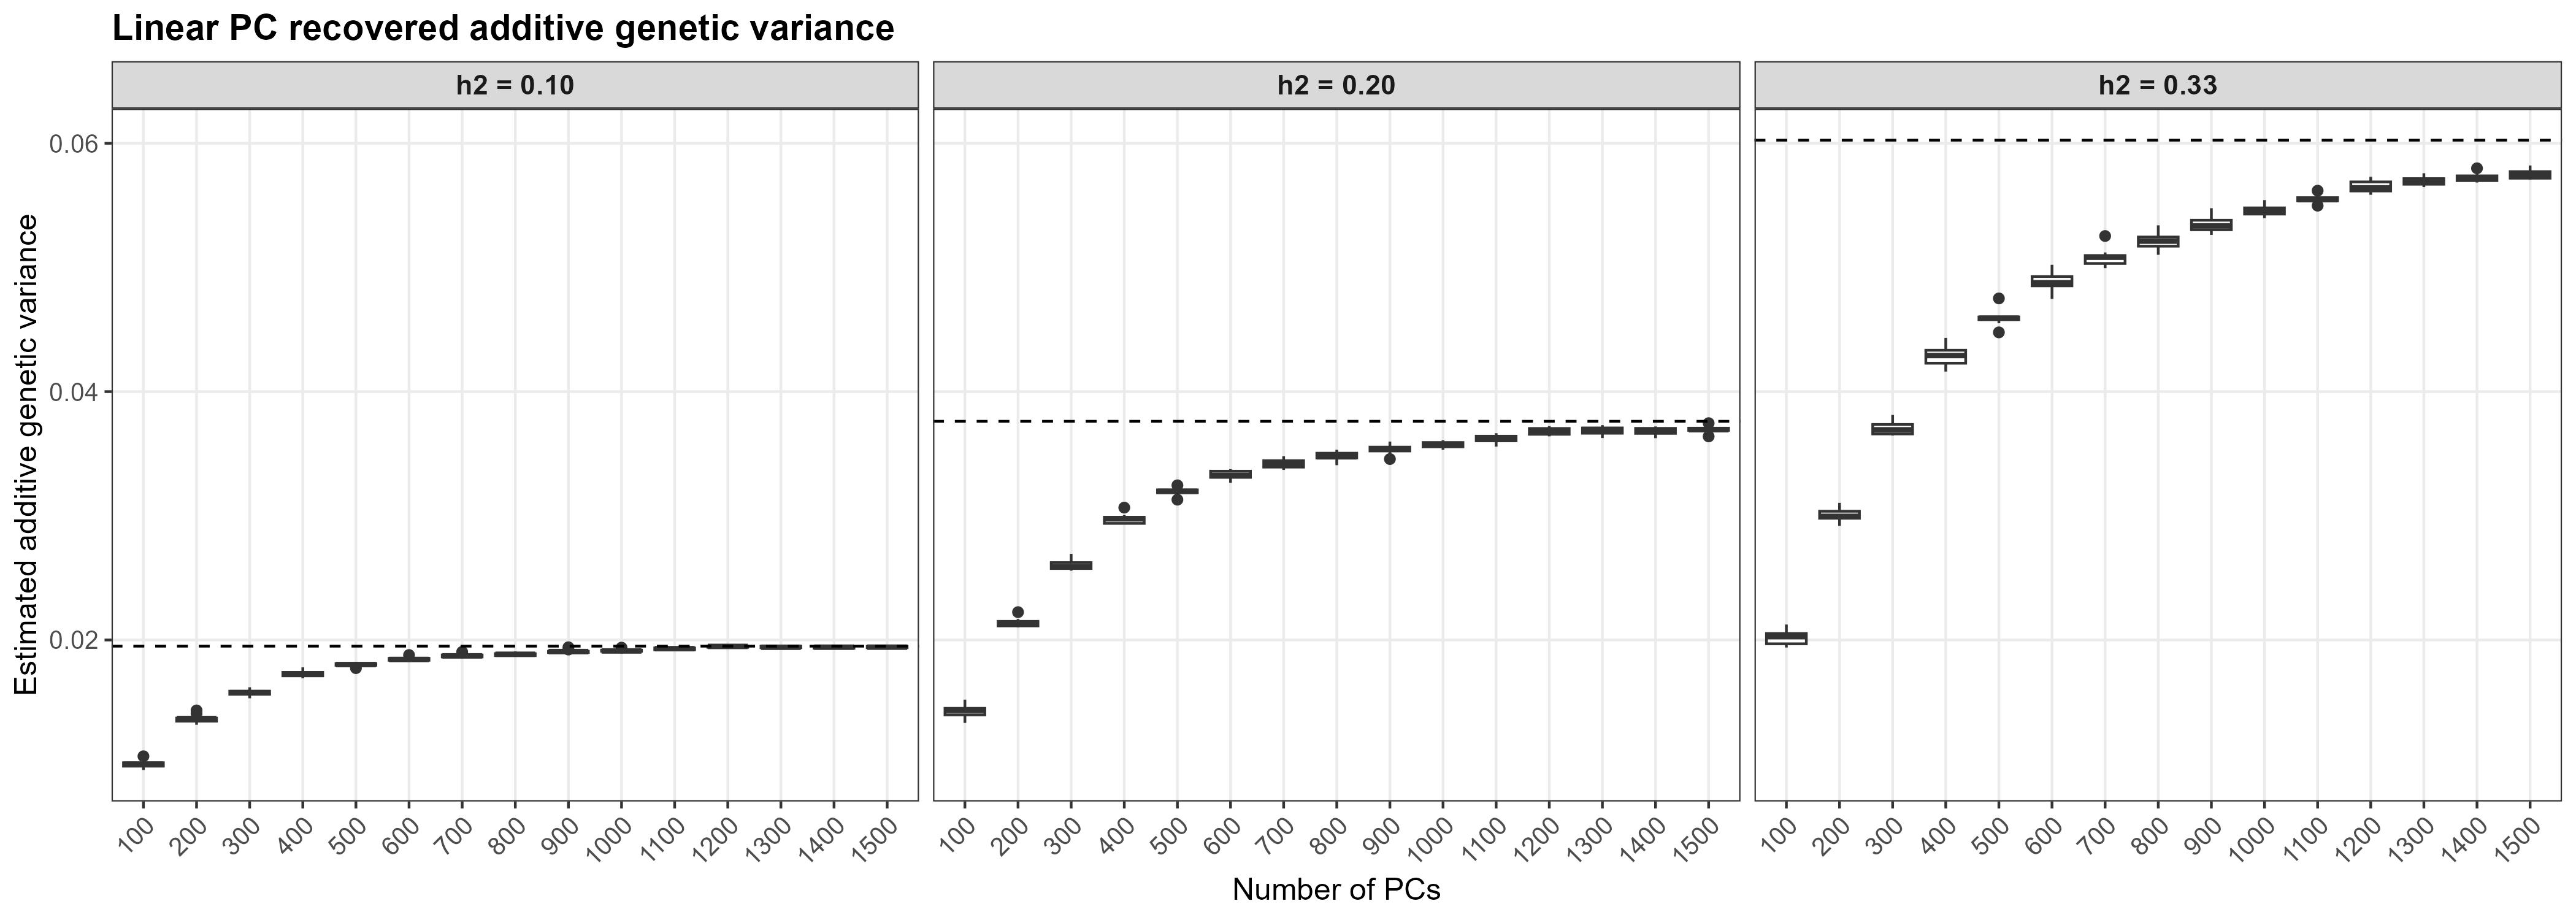
\includegraphics[width=\textwidth]{Figures/Results/simulations/additive_genetic_variance_vs_pc_combined.jpg}
        \caption{Recovered heritability by the linear model as a function of the number of principal components ($K$) for three heritability levels. Boxplots show the distribution across 10 independent replicates. The corresponding true observation-scale heritabilities are $0.078$, $0.150$, and $0.241$.}
        \label{fig:lin_h2_vs_K_h2}
    \end{subfigure}

    \caption[Recovered heritability for binary and linear models]{
    Recovered heritability as a function of the number of principal components ($K$) for the binary and linear models.
    }
    \label{fig:h2_vs_K_combined}
    \caption[Recovered heritability for binary and linear models]{
    Recovered heritability as a function of the number of principal components ($K$) for the binary and linear models.
    }
    \label{fig:h2_vs_K_combined}
\end{figure}

% ---------------- Runtime results ? --------------------

\section{Predicting dispersal in the Helgeland system }
%\todo[inline]{I would rename this, because the real data actually have a name (house sparrows and which trait you actually study, i.e., disperal). }

%\todo[inline]{Results are typically written in past tense, as in Section 4.1} 

The binary and linear BPCRR models were applied to the house sparrow data from the Helgeland system, and where the goal is to predict the binary trait dispersal. This included selecting the numbers of PCs to use, and comparing the predictive performance of the binary and linear models with the standard modeling approach in the field. Next, we compared the ranking of the individuals both with respect to the estimated breeding values and the predicted probability or score. Lastly, we did a robustness test for the estimated breeding values that were used down-stream for looking at fitness measures. 

We selected the number of PCs to use for both models by assessing predictive performance with the PR-AUC \autoref{fig:select_K_whole}). Both models achieved their highest PR-AUC at $K = 200$, with a PR-AUC of $0.41$ for the binary model and $0.40$ for the linear model. Compared with the prevalence in the data, which is $0.23$, this corresponded to a $78\%$ and $74\%$ improvement over a random classifier, respectively.
The PR-AUC were also relatively stable across all values of $K$. For the binary model, the lowest PR-AUC was observed at $K = 1400$, where it was $0.38$. For the linear model, the lowest value was observed at $K = 1500$, where it was $0.34$. These values still corresponded to improvements of $65\%$ and $48\%$, respectively, compared with a random classifier.

Considering runtime, we observed that it increased with $K$, as expected (\autoref{tab:runtime_selectk_pc}). The difference in runtime between the binary and linear models was generally small for each value of $K$, with neither model consistently being faster than the other.

In the following, when referring to the BPCRR models, we use the models with $K = 200$ for both the linear and binary models. These models will be used in the subsequent comparisons.

% ---------------------- Selecting K plots ----------------


% PR-AUC vs. K for linear and binary model 
\begin{figure}[htbp]
    \centering
    \begin{subfigure}[b]{0.49\textwidth}
        \centering
        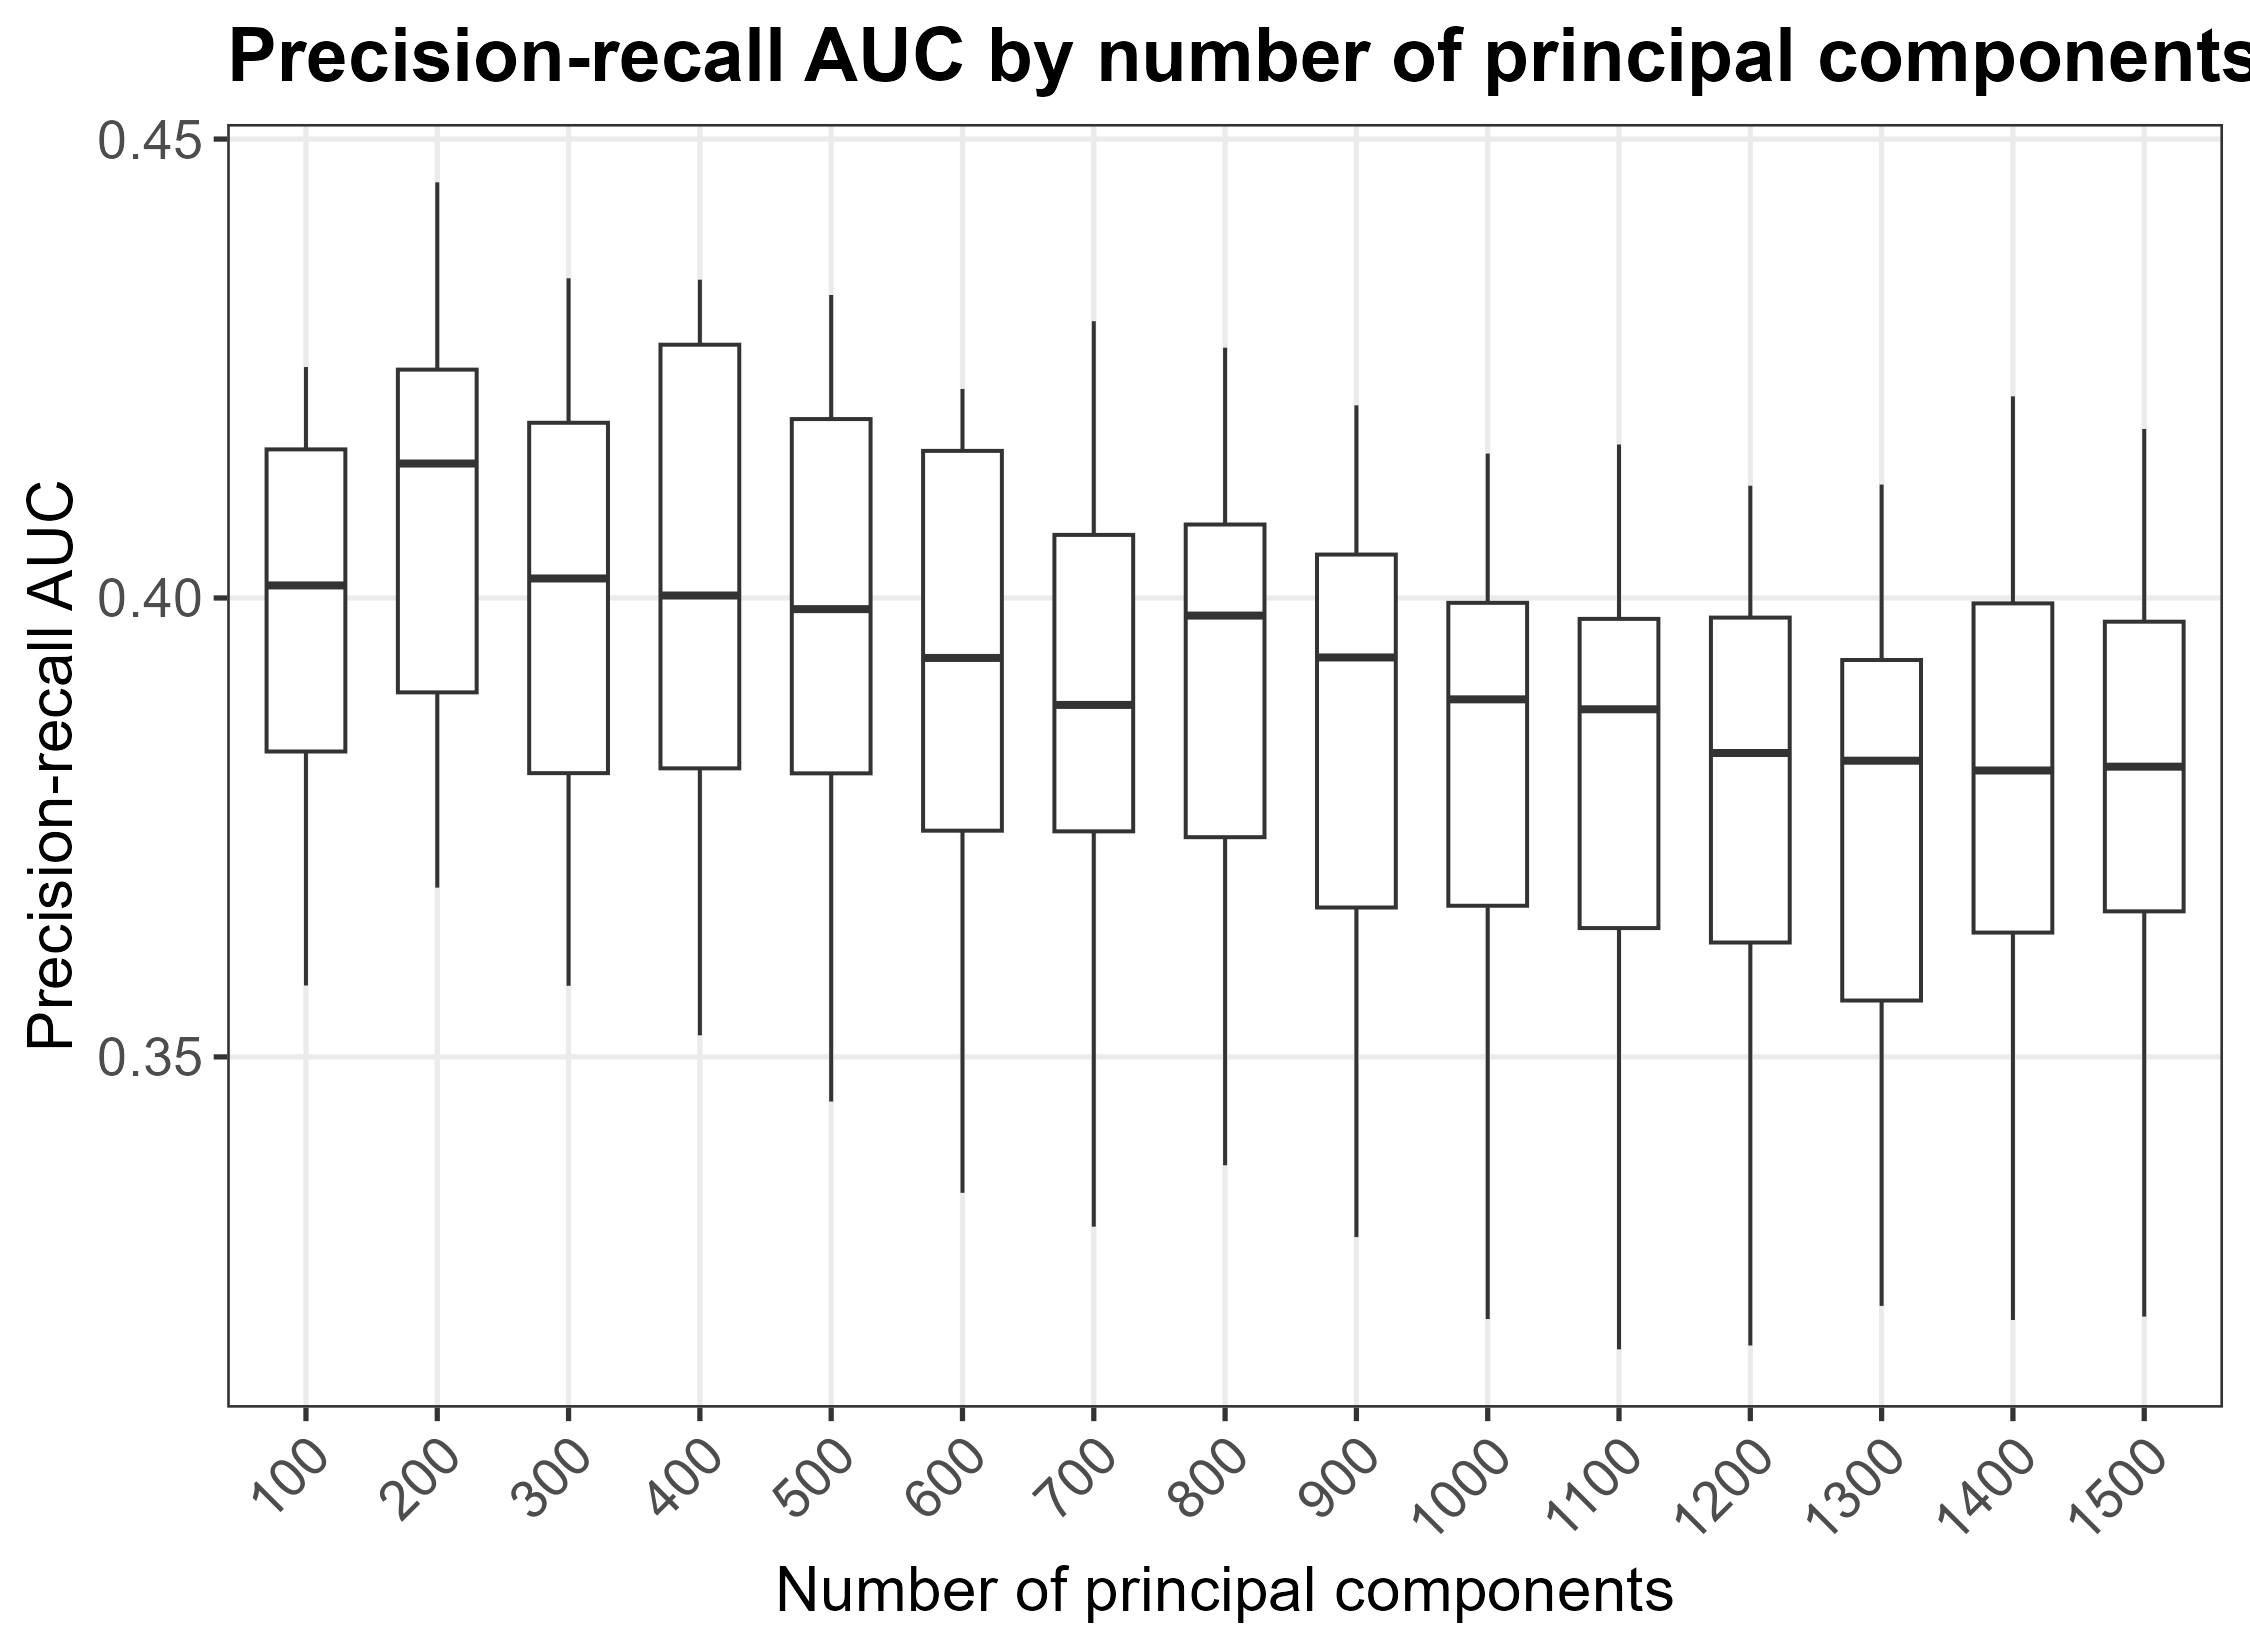
\includegraphics[width=\textwidth]{Figures/Results/real data/pr_auc_vs_k_26-03-05PC2_dropIsland61.png}
        \label{fig:bin_select_K}
    \end{subfigure}
    \hfill
    \begin{subfigure}[b]{0.49\textwidth}
        \centering
        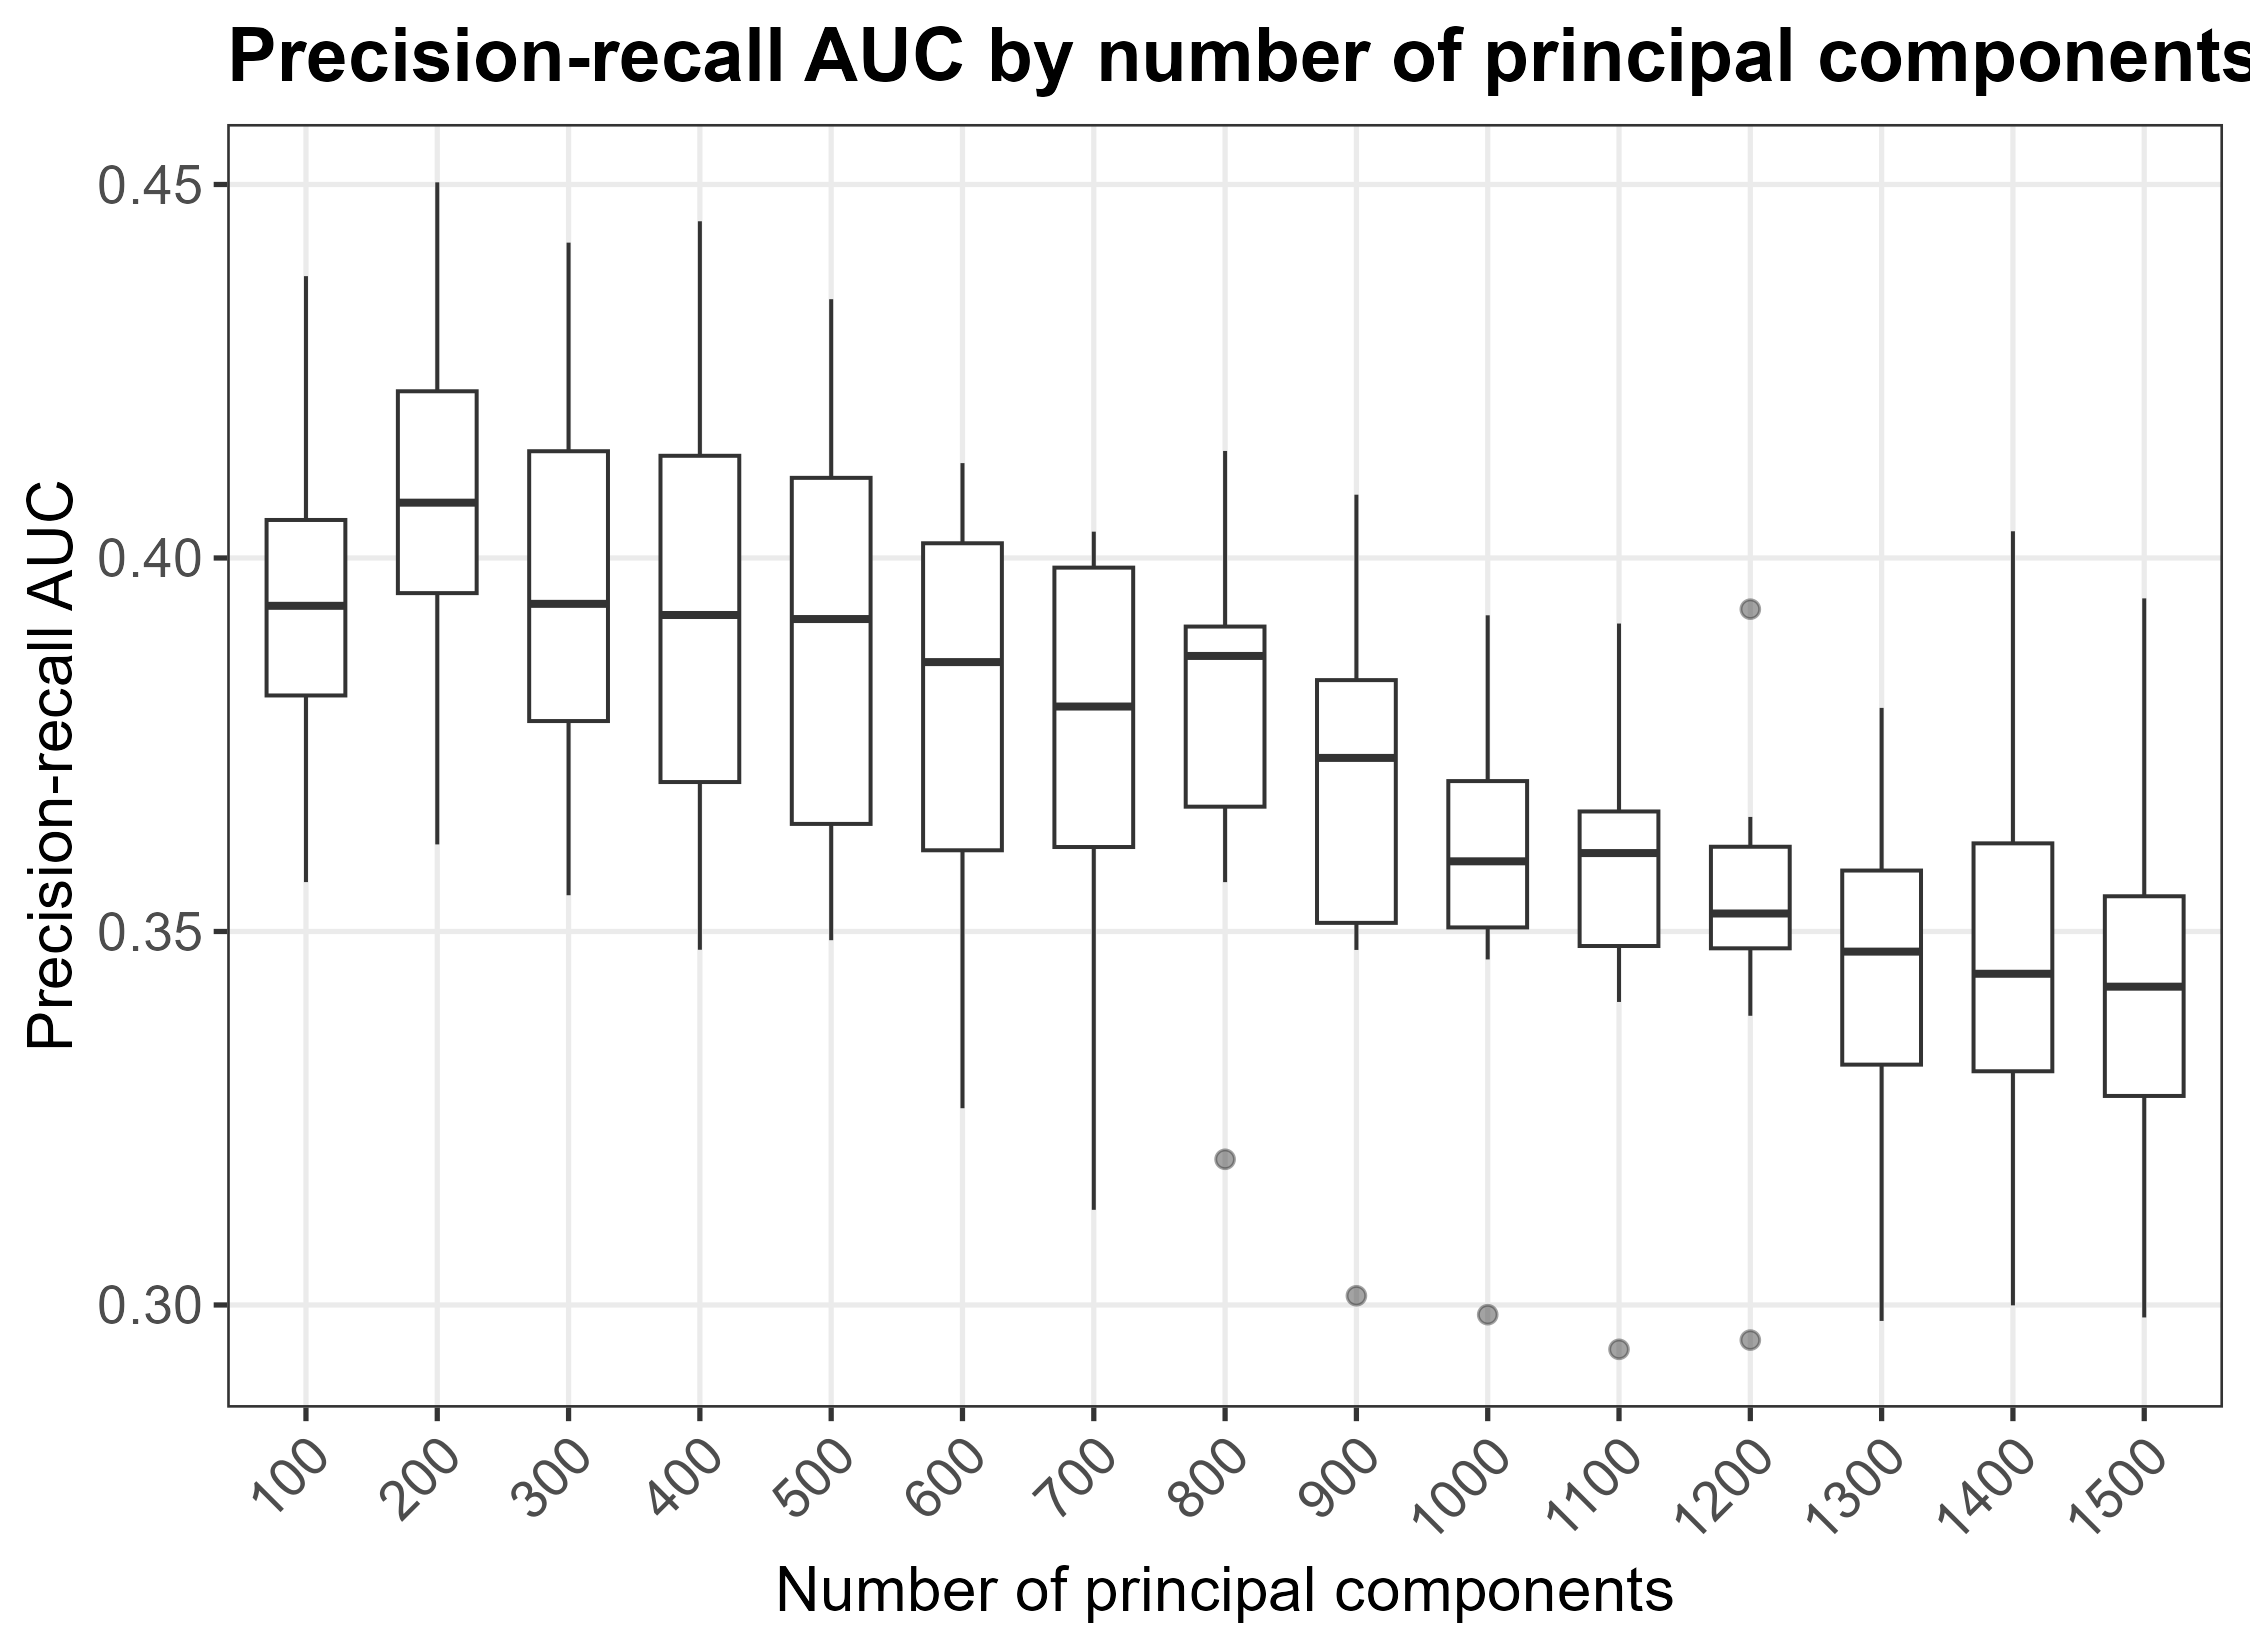
\includegraphics[width=\textwidth]{Figures/Results/real data/pr_auc_vs_k_26-03-17_LinPC1_dropIsland61.png}
        \label{fig:lin_select_K}
    \end{subfigure}
    
    \caption[Selecting number of principal components]{PR-AUC as a function of number of principal components for the binary model (left), and the linear model (right). Boxplots show the distribution across 10 independent replicates, with the horizontal line indicating the median PR-AUC.}
    \label{fig:select_K_whole}
\end{figure}

% runtimes, maybe for appendix? looks not so good in the pdf
\begin{table}[htbp]
  \centering
  \caption{Mean runtime for the binary and linear BPCRR models across the evaluated numbers of principal components, \(K\).
  Runtime is given in minutes and was averaged across 10 replicate runs for each value of \(K\).}
  \label{tab:runtime_selectk_pc}
  \begin{tabular}{rrr}
  \hline
  \(K\) & Binary PC mean runtime (min) & Linear PC mean runtime (min) \\
  \hline
  100  & 0.79  & 0.67 \\
  200  & 1.81  & 1.90 \\
  300  & 3.20  & 3.36 \\
  400  & 5.13  & 6.52 \\
  500  & 7.02  & 8.64 \\
  600  & 10.17 & 12.52 \\
  700  & 14.11 & 16.65 \\
  800  & 19.20 & 21.56 \\
  900  & 23.87 & 23.42 \\
  1000 & 32.50 & 31.41 \\
  1100 & 44.58 & 44.57 \\
  1200 & 55.36 & 60.60 \\
  1300 & 66.03 & 61.45 \\
  1400 & 82.13 & 78.20 \\
  1500 & 101.73 & 90.58 \\
  \hline
  \end{tabular}
  \end{table}


% --------- Compare with regualr GRM models results ----------------

The BPCRR models displayed comparable predictive performance to the standard animal models (GRM) that is commonly used in the field (\autoref{fig:all_models_compared}, \autoref{tab:highest_pr_auc_proportions}). The binary BPCRR and binary GRM models showed the highest median PR-AUC values, both around $0.41$, while the linear BPCRR and linear GRM models followed closely at around $0.40$. Thus, the differences in predictive performance were small. Interestingly, when looking at each rep and selecting the model with the highest PR-AUC the linear GRM model was selected in $40\%$ of the replicates, and the linear PC in $30\%$ of the replicates leaving only $30\%$ for the two binary models (\autoref{tab:highest_pr_auc_proportions}). However, the BPCRR models outperformed the standard GRM models in terms of runtime (\autoref{tab:runtime_dropisland61}). The binary and linear BPCRR models required $1.81$ and $1.90$ minutes, respectively, whereas the corresponding GRM models required $24.17$ and $21.57$ minutes.


% ---------- Compare with regular GRM models figures ----------------

\begin{figure}[htbp]
    \centering
    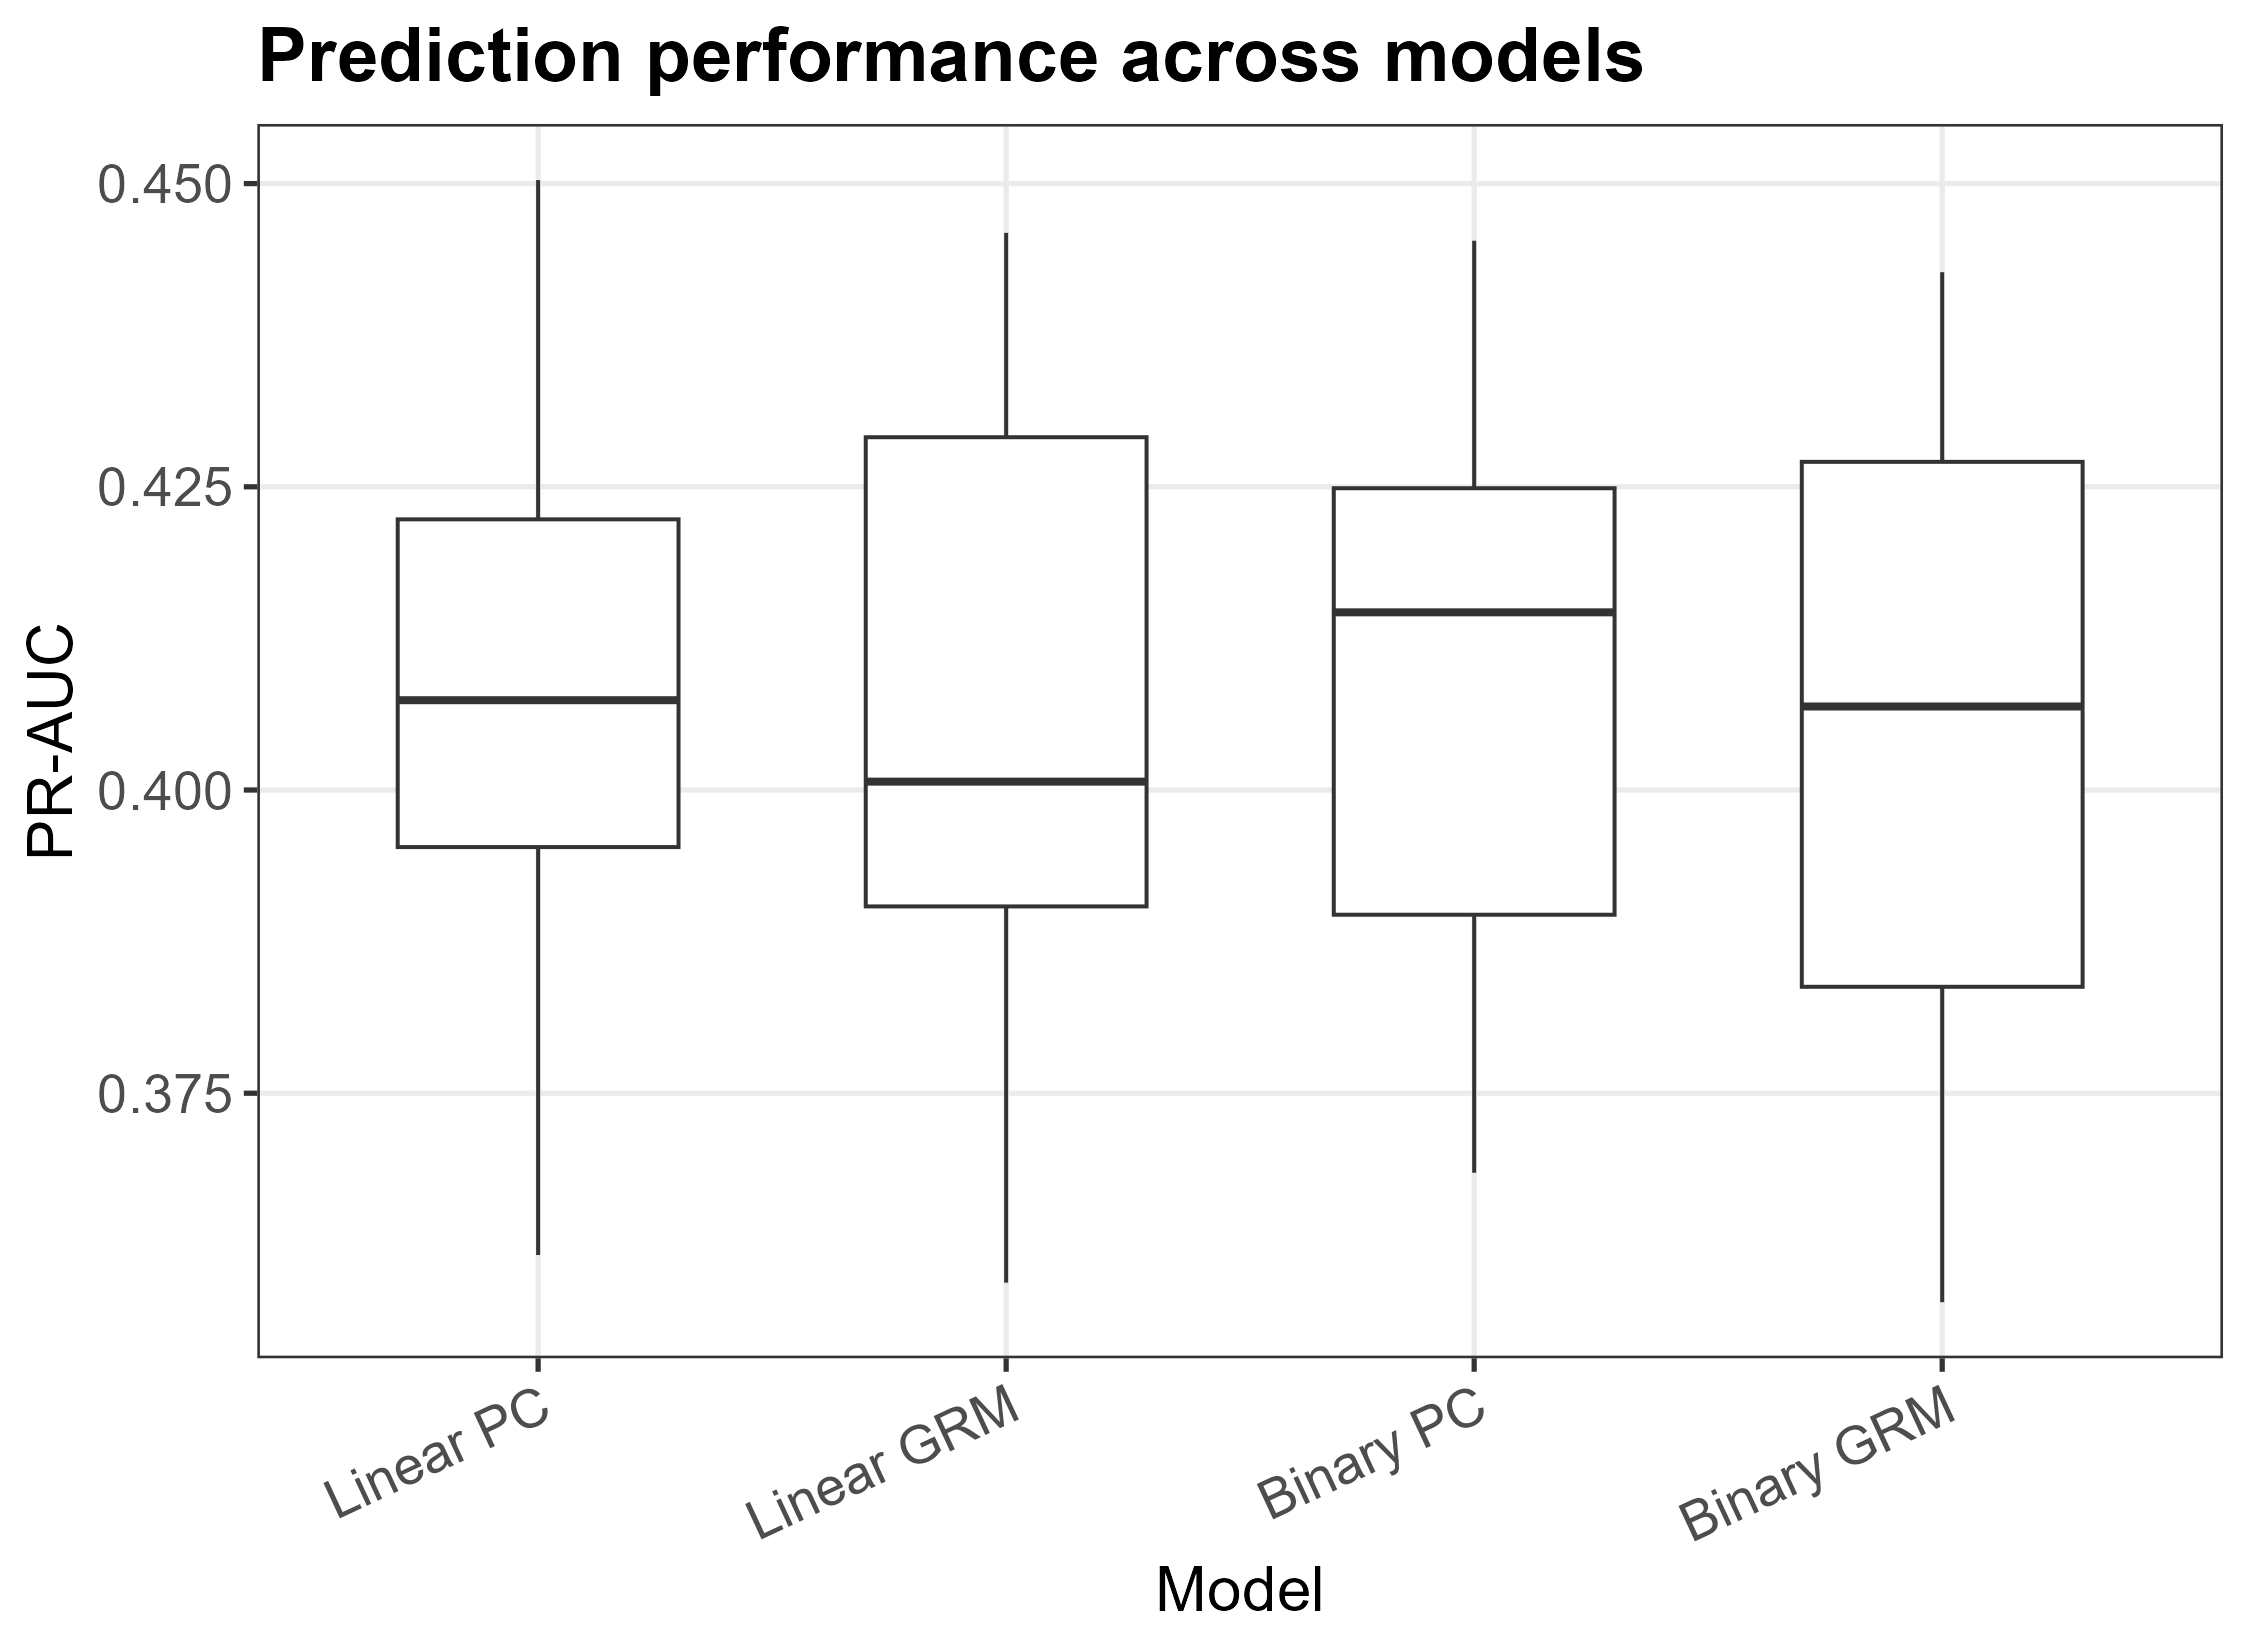
\includegraphics[width=\textwidth]{Figures/Results/real data/box_pr_auc.png}
    \caption[
    Comparing BPCRR and standard GRM
    ]{
    PR-AUC for all four models: binary and linear GRM, and BPCRR. The boxplots are summaries over 10 replications.  
    }

    \label{fig:all_models_compared}
\end{figure}

% pop of reps with higest pr-auc 
\begin{table}[htbp]
      \centering
      \caption{Proportion of replicates where each model had the highest PR-AUC. The total number of replicates was $10$.}
      \label{tab:highest_pr_auc_proportions}
      \begin{tabular}{lc}
          \hline
          Model & Proportion of replicates \\
          \hline
          Linear PC  & 0.30 \\
          Linear GRM & 0.40 \\
          Binary PC  & 0.20 \\
          Binary GRM & 0.10 \\
          \hline
      \end{tabular}
  \end{table}

% runtime table 

\begin{table}[htbp]
  \centering
  \caption{Mean runtime for the four models included in the comparison. Runtime was averaged across the 10
  replicate runs for each model. For the two principal component (PC) models, the number of PCs was fixed at \(K = 200\).}
  \label{tab:runtime_dropisland61}
  \begin{tabular}{lr}
  \hline
  Model & Mean runtime (min) \\
  \hline
  Binary PC & 1.81 \\
  Linear PC & 1.90 \\
  Binary GRM & 24.17 \\
  Linear GRM & 21.57 \\
  \hline
  \end{tabular}
  \end{table}

% --- correlation between binary and linear breeding values and responses

When examining the ranking of individuals, we observed a clear correspondence between the binary and linear predictions (\autoref{fig:bpcrr_comparison}). The estimated breeding values aligned closely between the two models, with a Spearman's rho of $0.951$ (\autoref{fig:bpcrr_comparison}), where a value of $1.0$ would indicate perfect agreement in ranking. 
Individuals with high breeding values for dispersal tended to have dispersed, whereas individuals with low breeding values tended not to have dispersed, but the separation of the groups was not very clear.  
At the same time, there appeared to be a subgroup of individuals located somewhat off the diagonal, with relatively higher breeding values under the linear model than under the binary model.
%
Inspection of this subgroup in the breeding value plots (diagnostic plots should be added to the appendix) showed that it included individuals from seven islands, with almost $80\%$ originating from island 38 (Aldra). Fewer than $10\%$ of the individuals in this group had dispersed, which was less than half the proportion observed in the full dataset ($23\%$). In addition, individuals from this island appeared to have a substantially higher inbreeding coefficient than the overall level in the data.
%
The predicted linear score and probability showed, on the other hand, stronger agreement, with a Spearman's rho of $0.941$. There appeared to be more variation between the binary and the linear model predicted score and probability for lower values than for higher values. 
%The points appeared to form two groups: a main cluster close to the diagonal, and a smaller subgroup with somewhat higher predicted scores under the linear model than under the binary model, particularly at the lower end of the score range. 
The separation between the two classes ($0/1$) appeared slightly clearer for the predicted dispersal scores than for the breeding values, although substantial overlap remained.
%add the diagnostics plots here in the appendix?


% -------------- correlation bin vs. lin figures -----------------
\begin{figure}[htbp]
    \centering
    
    \begin{subfigure}[t]{0.49\textwidth}
        \centering
        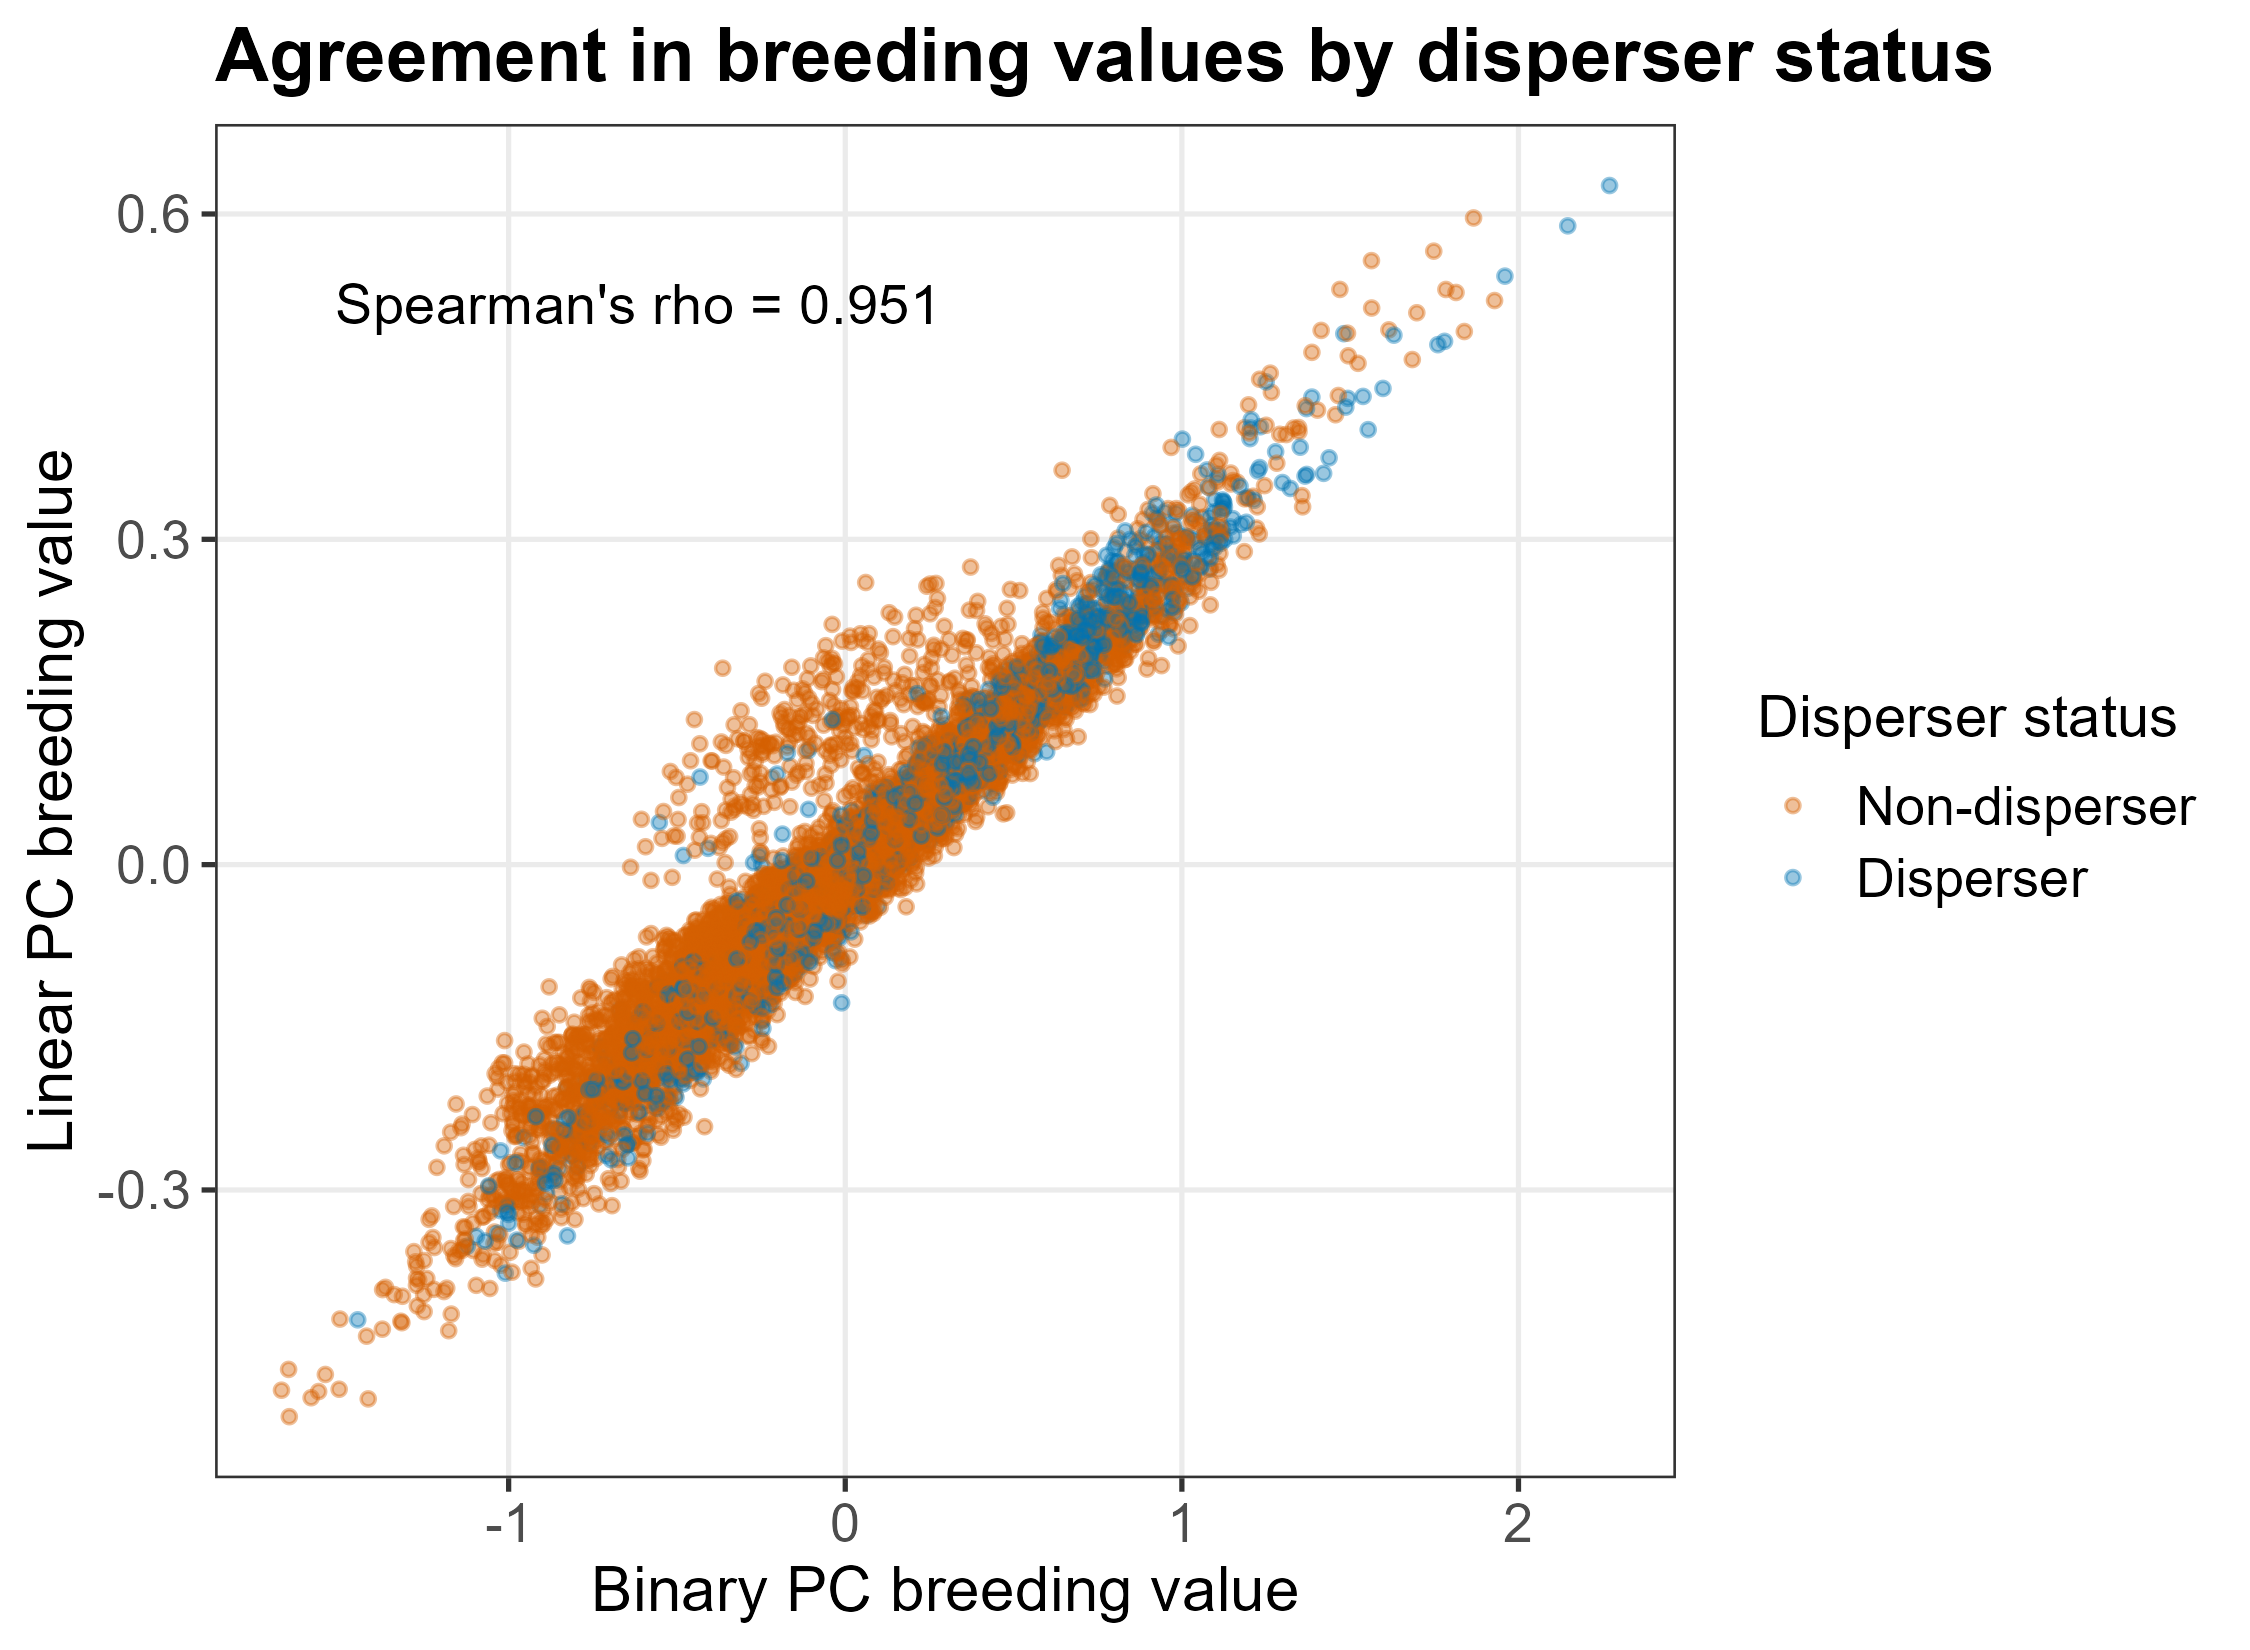
\includegraphics[width=\linewidth]{Figures/Results/real data/bin_vs_lin_pc_spearman_breeding_values_by_response.png}
    \end{subfigure}
    \hfill
    \begin{subfigure}[t]{0.49\textwidth}
        \centering
        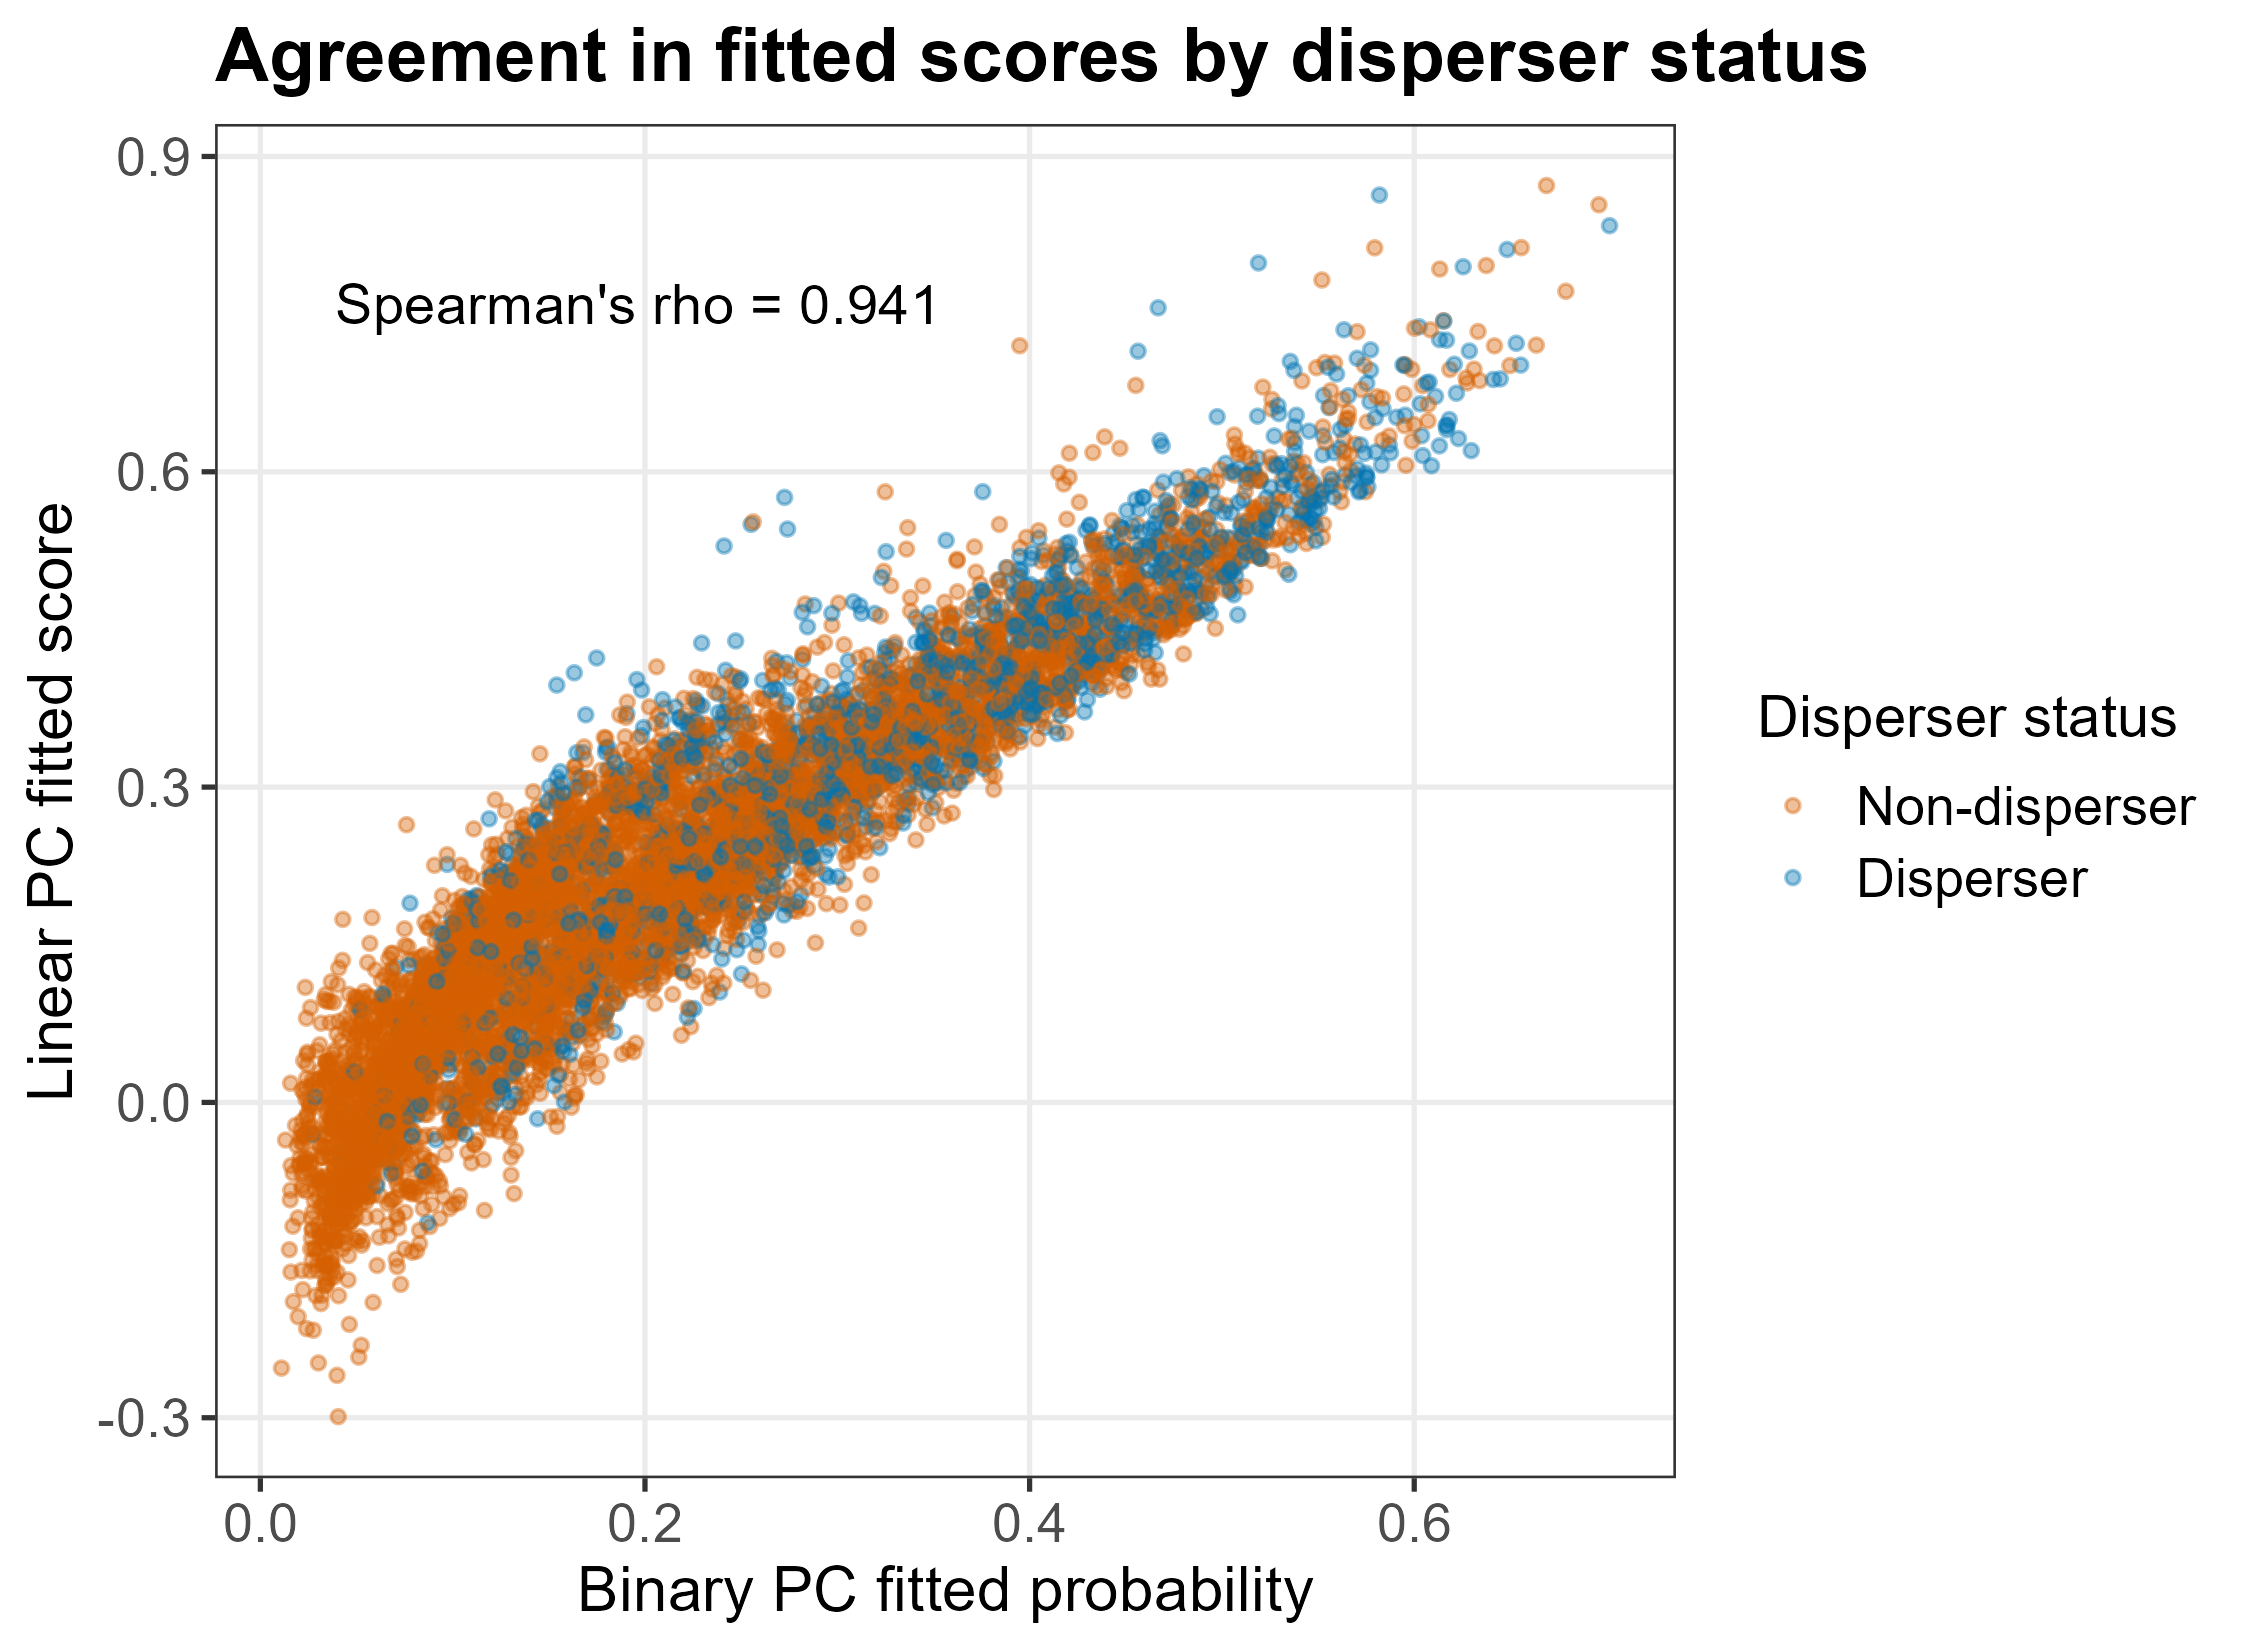
\includegraphics[width=\linewidth]{Figures/Results/real data/bin_vs_lin_pc_spearman_scores_by_response.png}
    \end{subfigure}
    
    \caption[Comparison of binary and linear BPCRR results]%
    {Comparison of binary and linear BPCRR results for the two model outputs. 
    The left panel shows breeding values from the binary and linear BPCRR models, 
    while the right panel shows the corresponding fitted scores or probabilities. 
    In both cases, the plots indicate a strong positive association between the two modeling approaches, 
    with Spearman's rho equal to 0.951 for breeding values and 0.941 for fitted scores.}
    \label{fig:bpcrr_comparison}
\end{figure}

% ------ distributions results ---------------

%distribution of BVs
One of the clearest differences between the binary and Gaussian models is the range of the estimated breeding values (\autoref{fig:dist_BVs}). The breeding values from the binary model range from approximately $-2$ to $2$, whereas those from the Gaussian model range from approximately $-0.4$ to $0.6$. This narrower range in the Gaussian model results in a more compressed density distribution, with higher modes for both true dispersers and true non-dispersers compared with the corresponding distributions from the binary model.
%
For both models, there is substantial overlap between true dispersers and true non-dispersers with respect to estimated breeding values. However, the distribution for true dispersers is shifted slightly to the right in both cases, indicating somewhat higher estimated breeding values among individuals that dispersed. The separation between the two groups remains limited, as both modes are located close to zero on the x-axis.    

%dist est pred
The distributions of the estimated dispersal probabilities from the binary model and the predicted linear scores from the Gaussian model show differences between the two approaches, but also some similarities (\autoref{fig:pred_density}). In both models, there is substantial overlap between true dispersers and true non-dispersers, indicating that the models do not fully separate the two groups.
%binary 
For the binary model, the distribution for true non-dispersers is relatively narrow and concentrated near an estimated dispersal probability of zero, with a tail extending towards probabilities close to one. The distribution for true dispersers is broader and the mode is shifted to the right compared to the non-dispersers, although the separation between the groups remains limited. Notably, the modal estimated probability for true dispersers is approximately $0.25$, and no individuals in the test set are assigned an estimated dispersal probability above $0.7$.
%linear model
For the Gaussian model, the distributions of prediction scores for true dispersers and true non-dispersers are more similar in shape, but the distribution for true dispersers is shifted towards higher prediction value. The true non-dispersers have a mode close to $0.0$, whereas the true dispersers have a mode of approximately $0.3$, with the two modes having similar heights. The range of prediction scores also differs from the range of estimated probabilities produced by the binary model, extending from approximately $-0.3$ to $0.9$.  




% --------- distribution of the predicted score and the probability and bredding values  ----------

%dist of BVs
\begin{figure}[htbp]
      \centering
      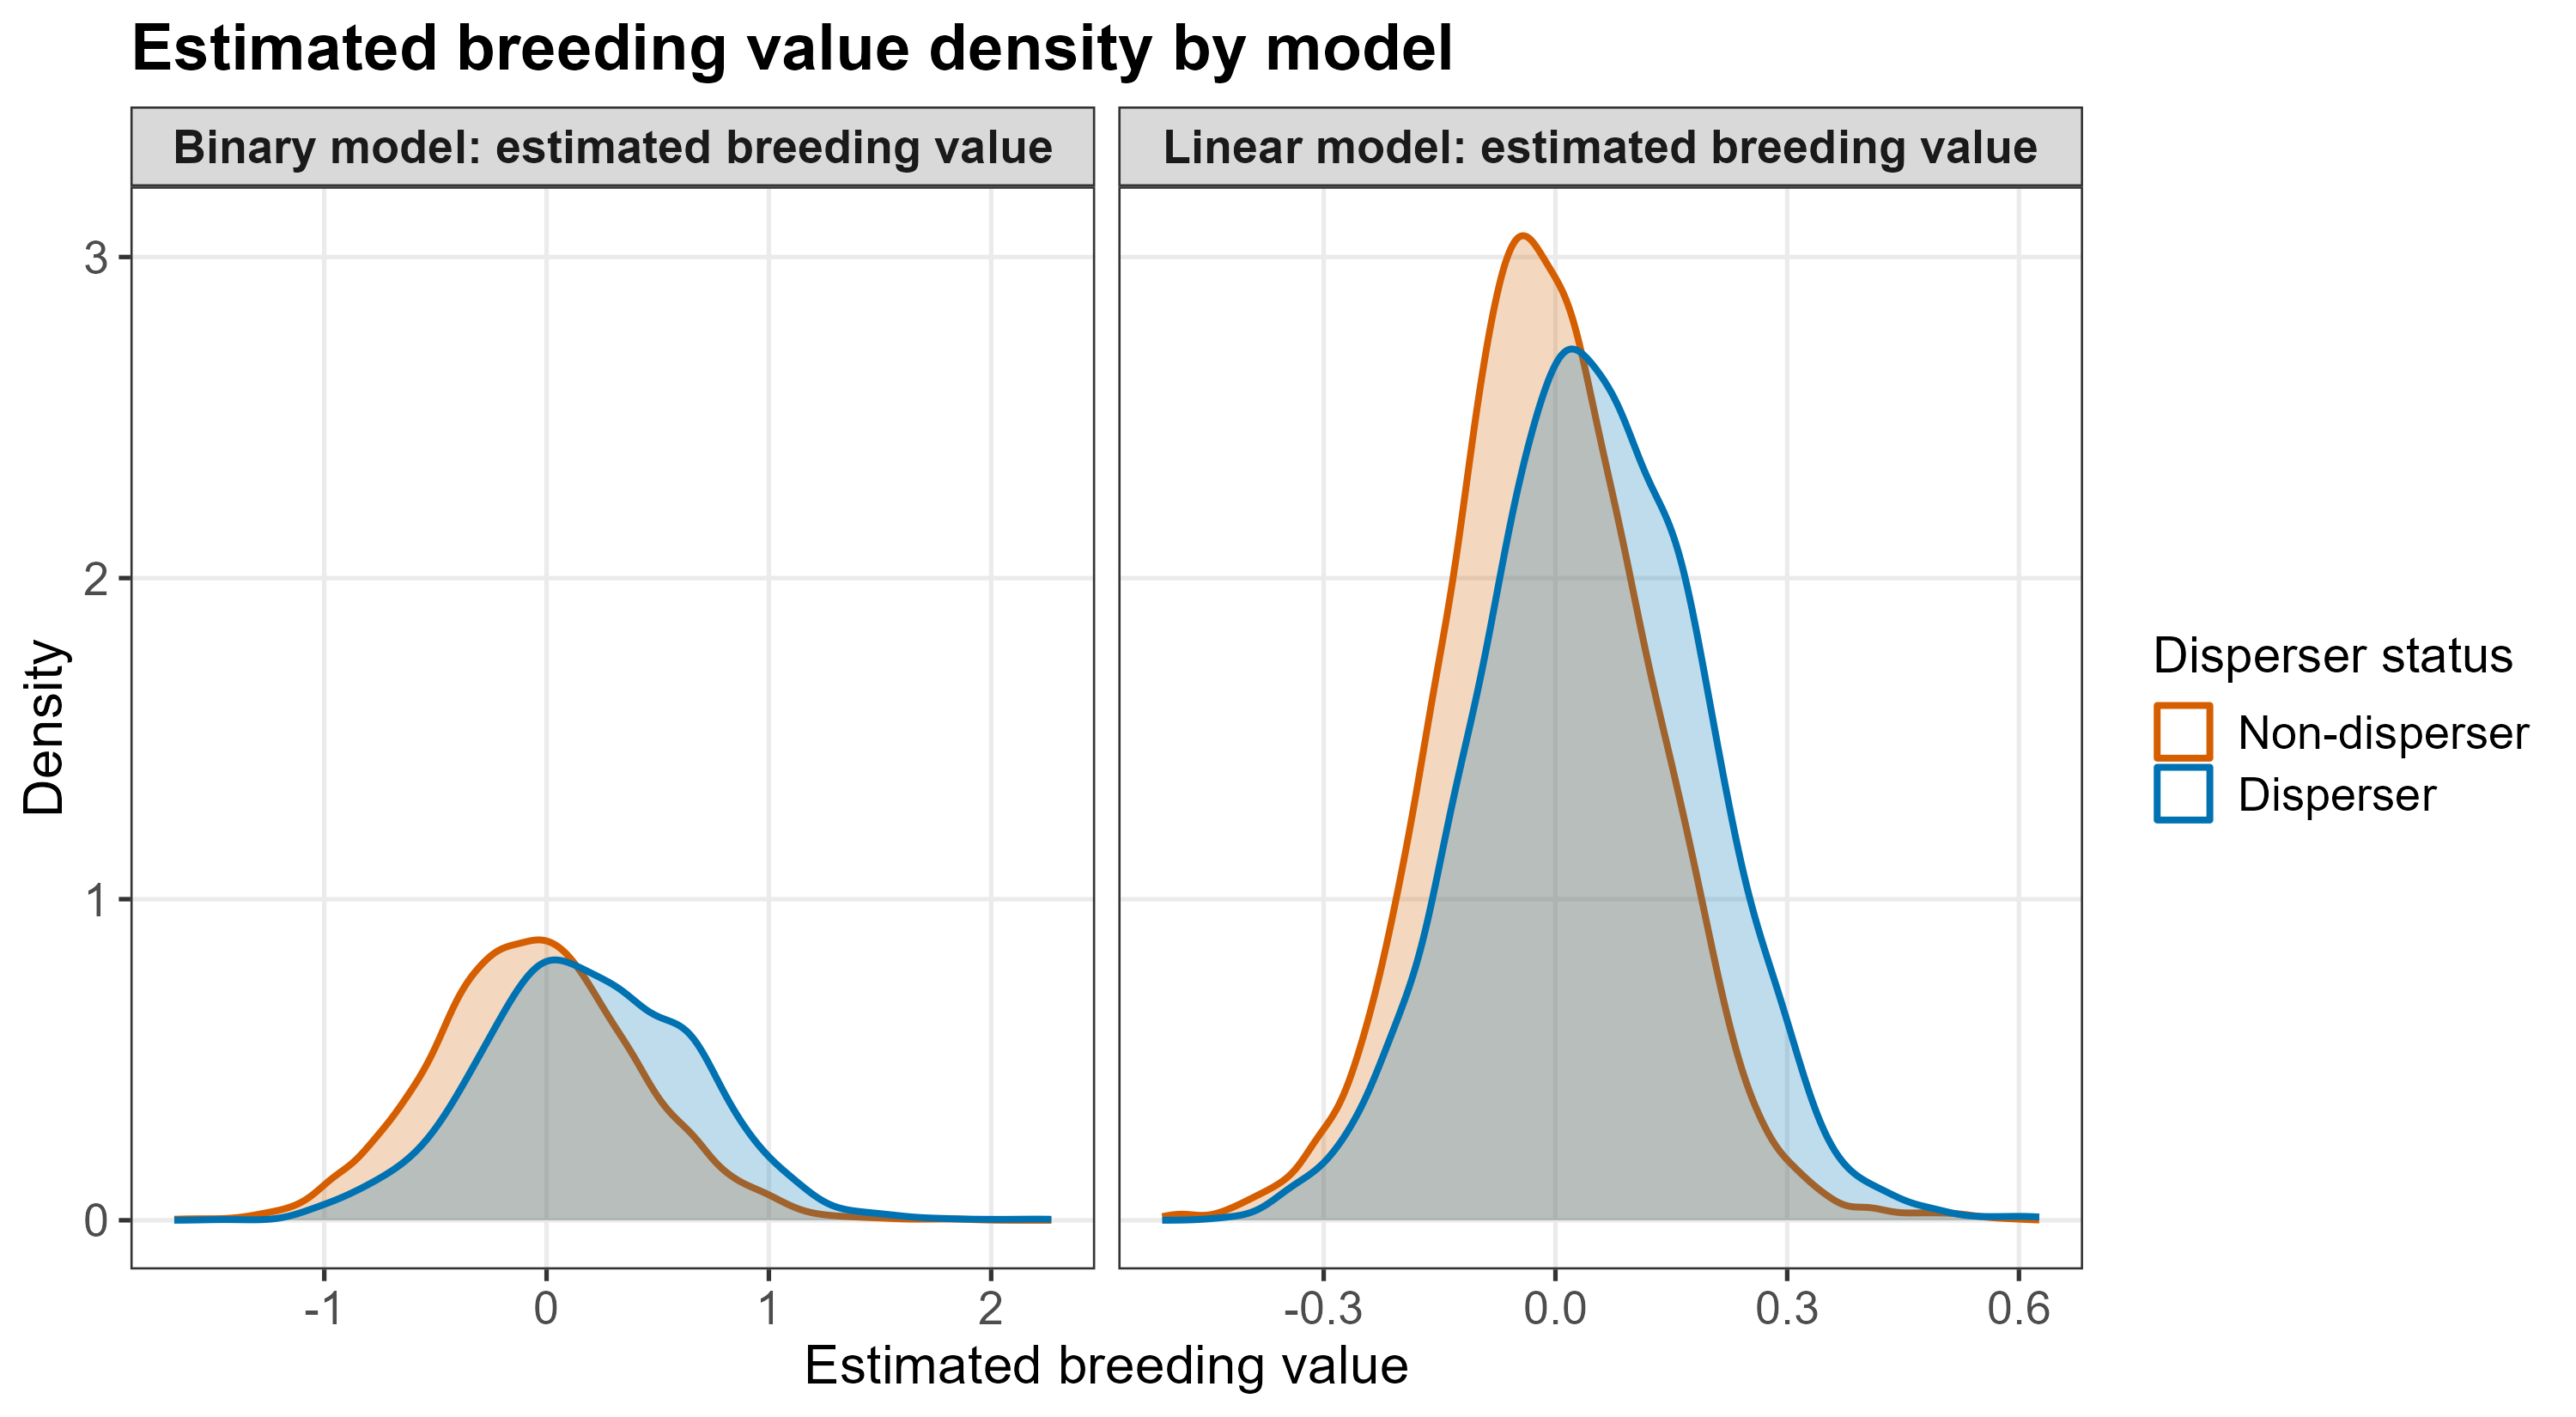
\includegraphics[width=\textwidth]{Figures/Results/real data/binary_linear_breeding_value_density_panels_by_y.png}
      \caption[Test set breeding value distributions] {Distributions of estimated breeding values from the binary and linear BPCRR models for the true dispersers and non-dispersers in the test set of the $10$ replicates.}
      \label{fig:dist_BVs}
  \end{figure}


%dist of pred scores 
\begin{figure}[htbp]
      \centering
      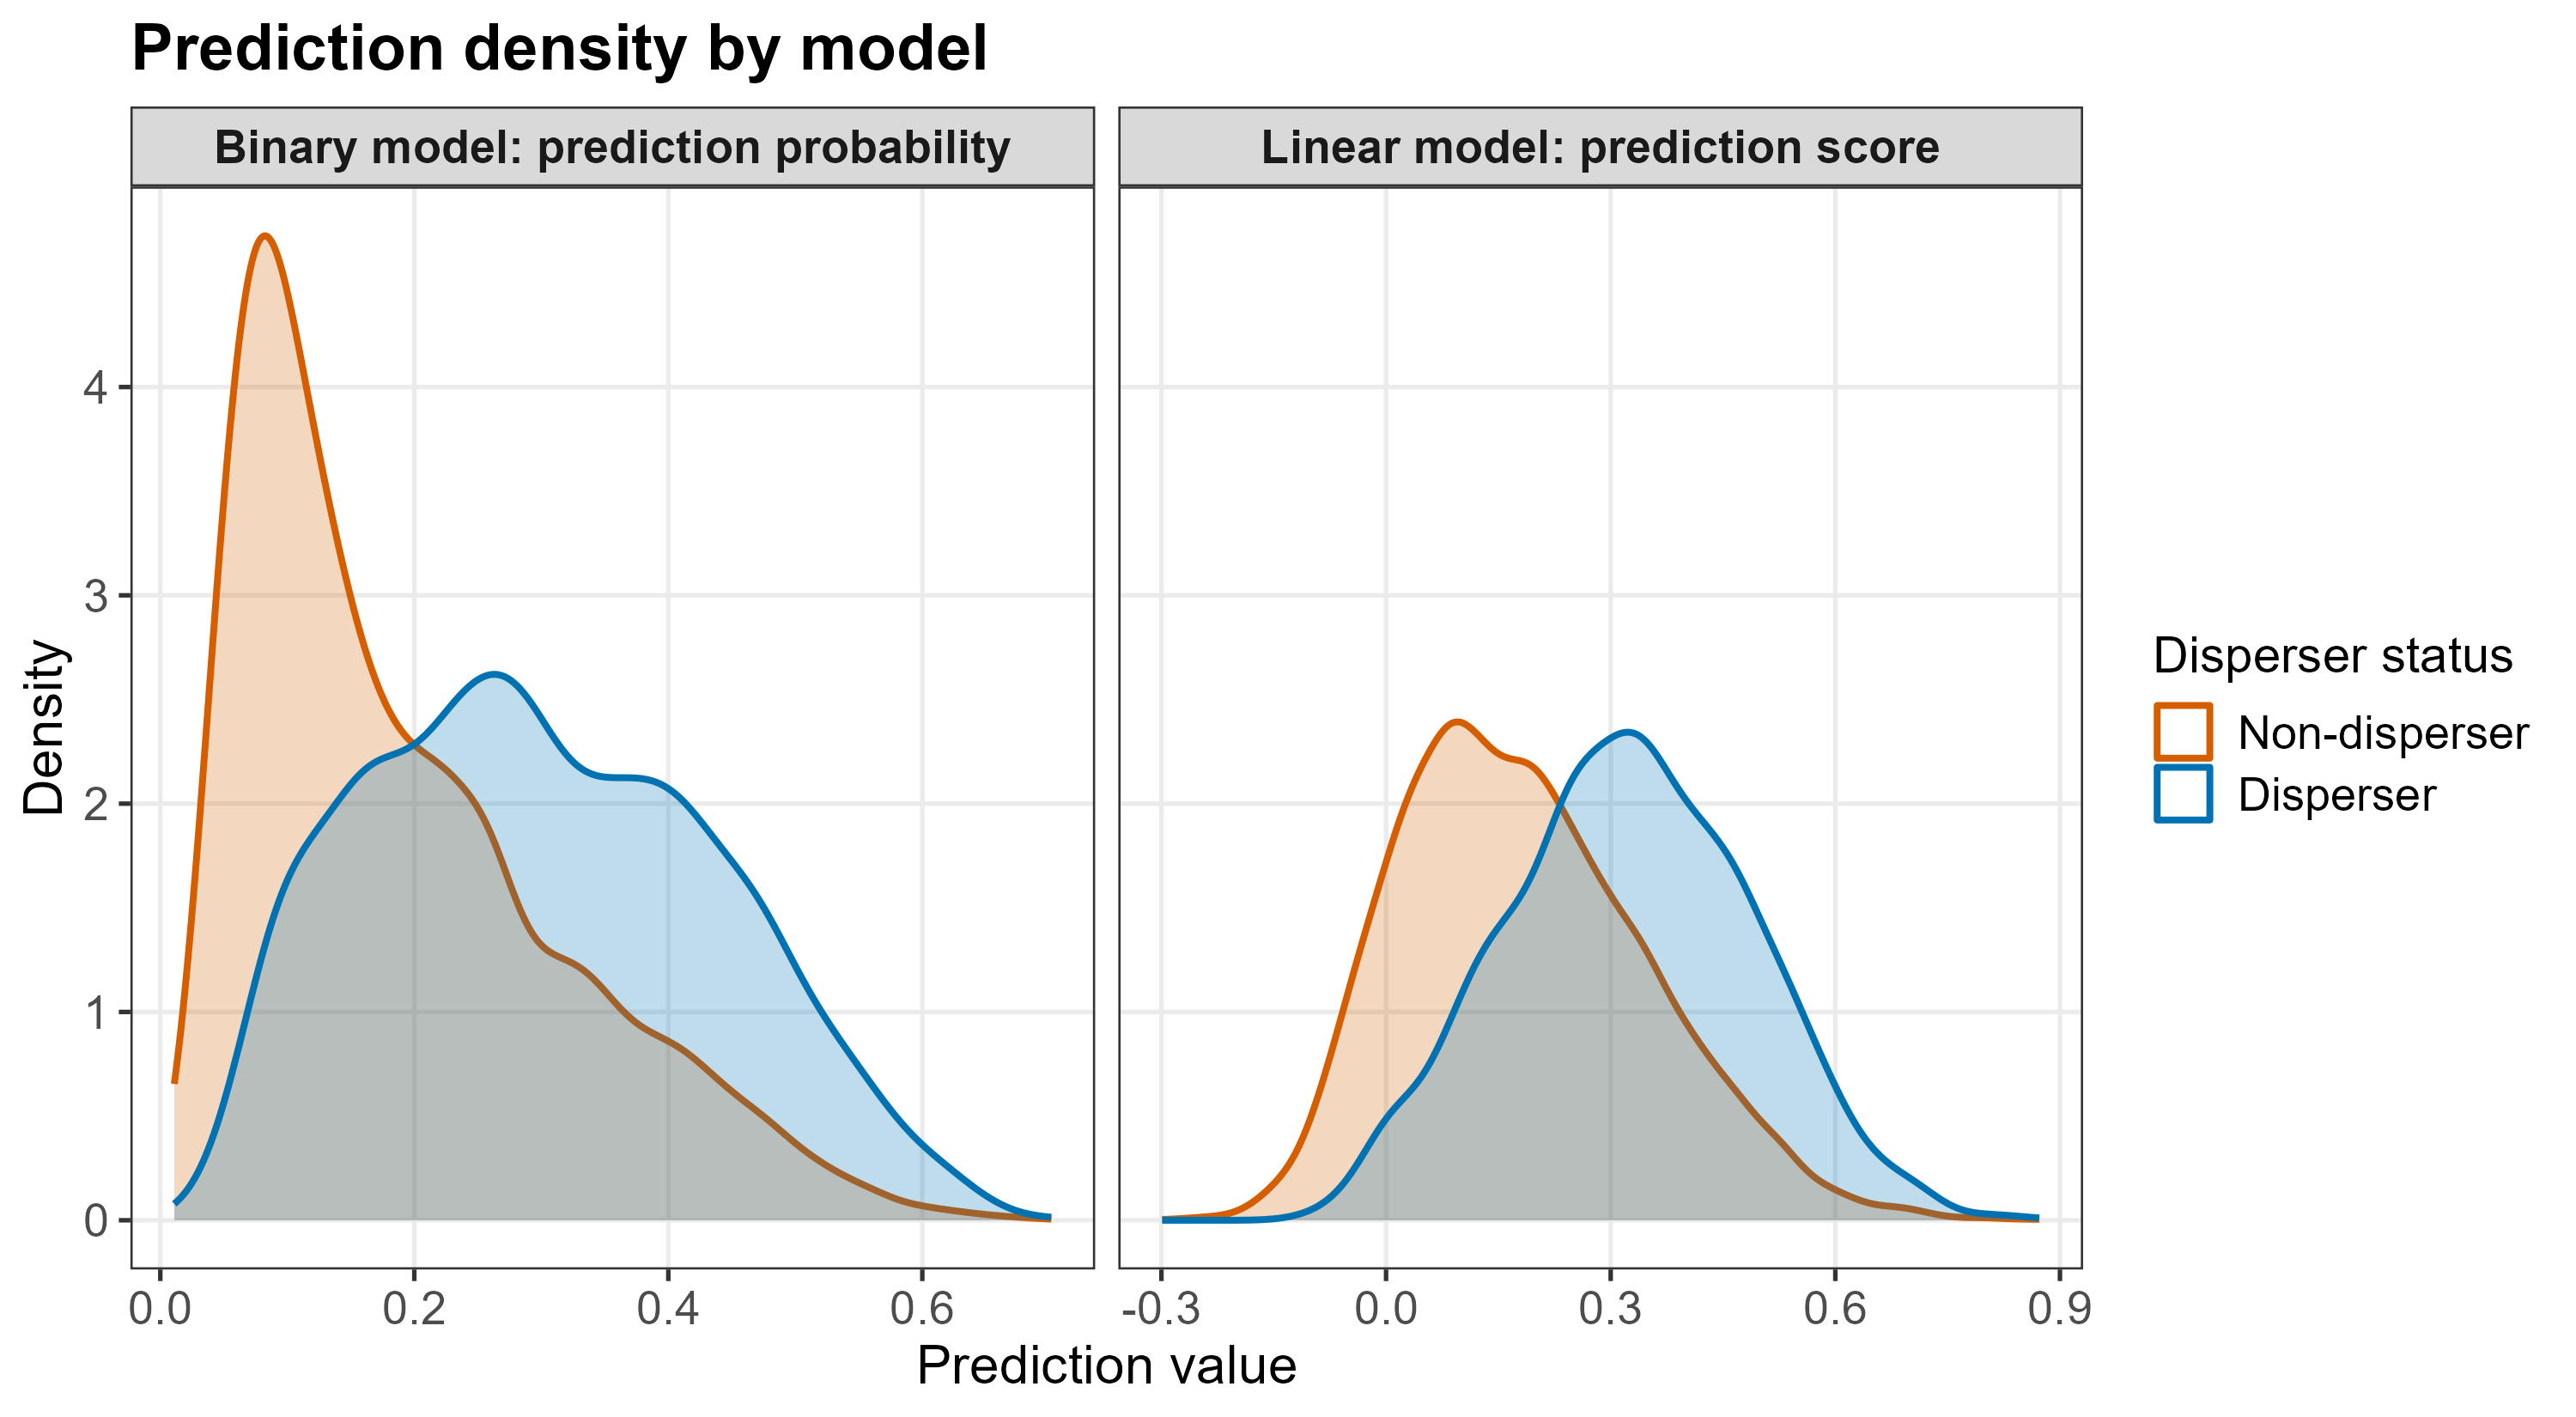
\includegraphics[width=\textwidth]{Figures/Results/real data/binary_linear_prediction_density_panels_by_y.png}
      \caption[Test set probability distributions] {Distributions of prediction probability and prediction score from the binary and linear BPCRR models for the true dispersers (blue) and non-dispersers (red) in the test set of the $10$ replicates.}
      \label{fig:dist_pred_scores}
  \end{figure}


% -------------- Robustness test? --------------------
\subsubsection*{Robustness test - move to methods instead}

Additional structure in the data became apparent during model assessment. As shown in \autoref{fig:pred_density}, the density of dispersing individuals was bimodal, with one subgroup showing substantially higher predicted probabilities of dispersal than the rest. All individuals in this subgroup originated from island 61 (Vega), which lies outside the study system, although they had all dispersed into the island system under study. To evaluate the influence of this subgroup, the binary PC model was fitted both with and without individuals from island 61. Model performance was then compared using only individuals included in both analyses, that is, excluding individuals from island 61 from the test sets (\autoref{fig:remove_island61}). The model trained without individuals from island 61 showed a slightly higher median PR-AUC, and the variation in PR-AUC was also somewhat smaller.  

% ------------- Removing Vega = Island 61 from the data ------
%maybe move to the appendix? 

\begin{figure}[htbp]
    \centering

    \begin{subfigure}[t]{0.49\textwidth}
        \centering
        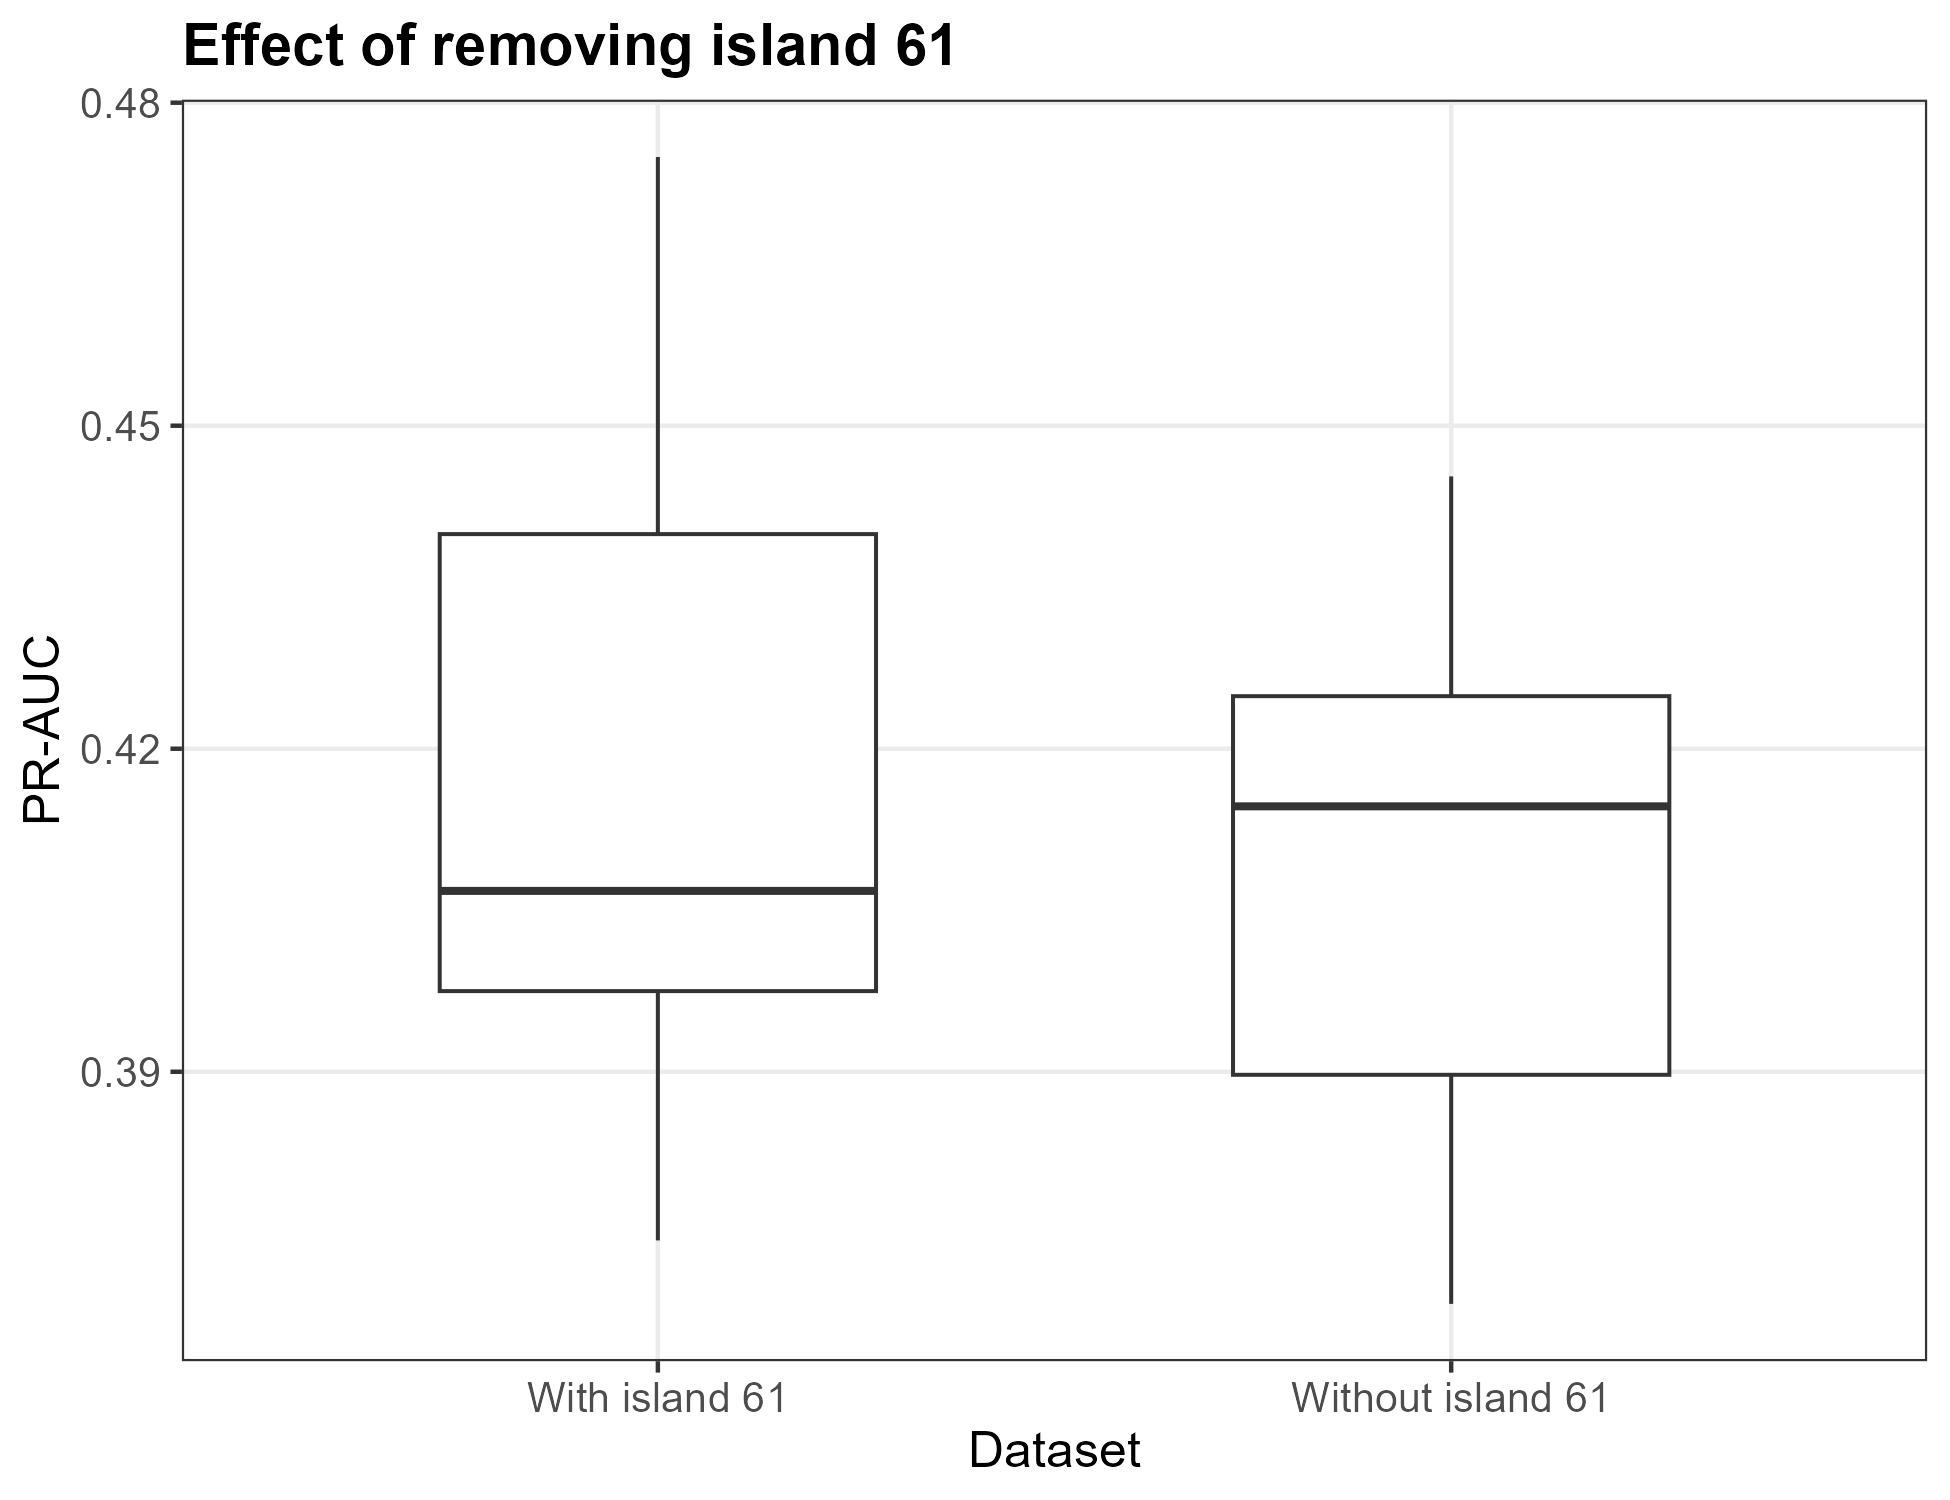
\includegraphics[width=\textwidth]{Figures/Results/real data/dropIsland61_vs_PC1_box_pr_auc.png}
        \caption{PR-AUC for the best binary PC model with and without individuals from island 61 (Vega).}
        \label{fig:remove_island61}
    \end{subfigure}
    \hfill
    \begin{subfigure}[t]{0.49\textwidth}
        \centering
        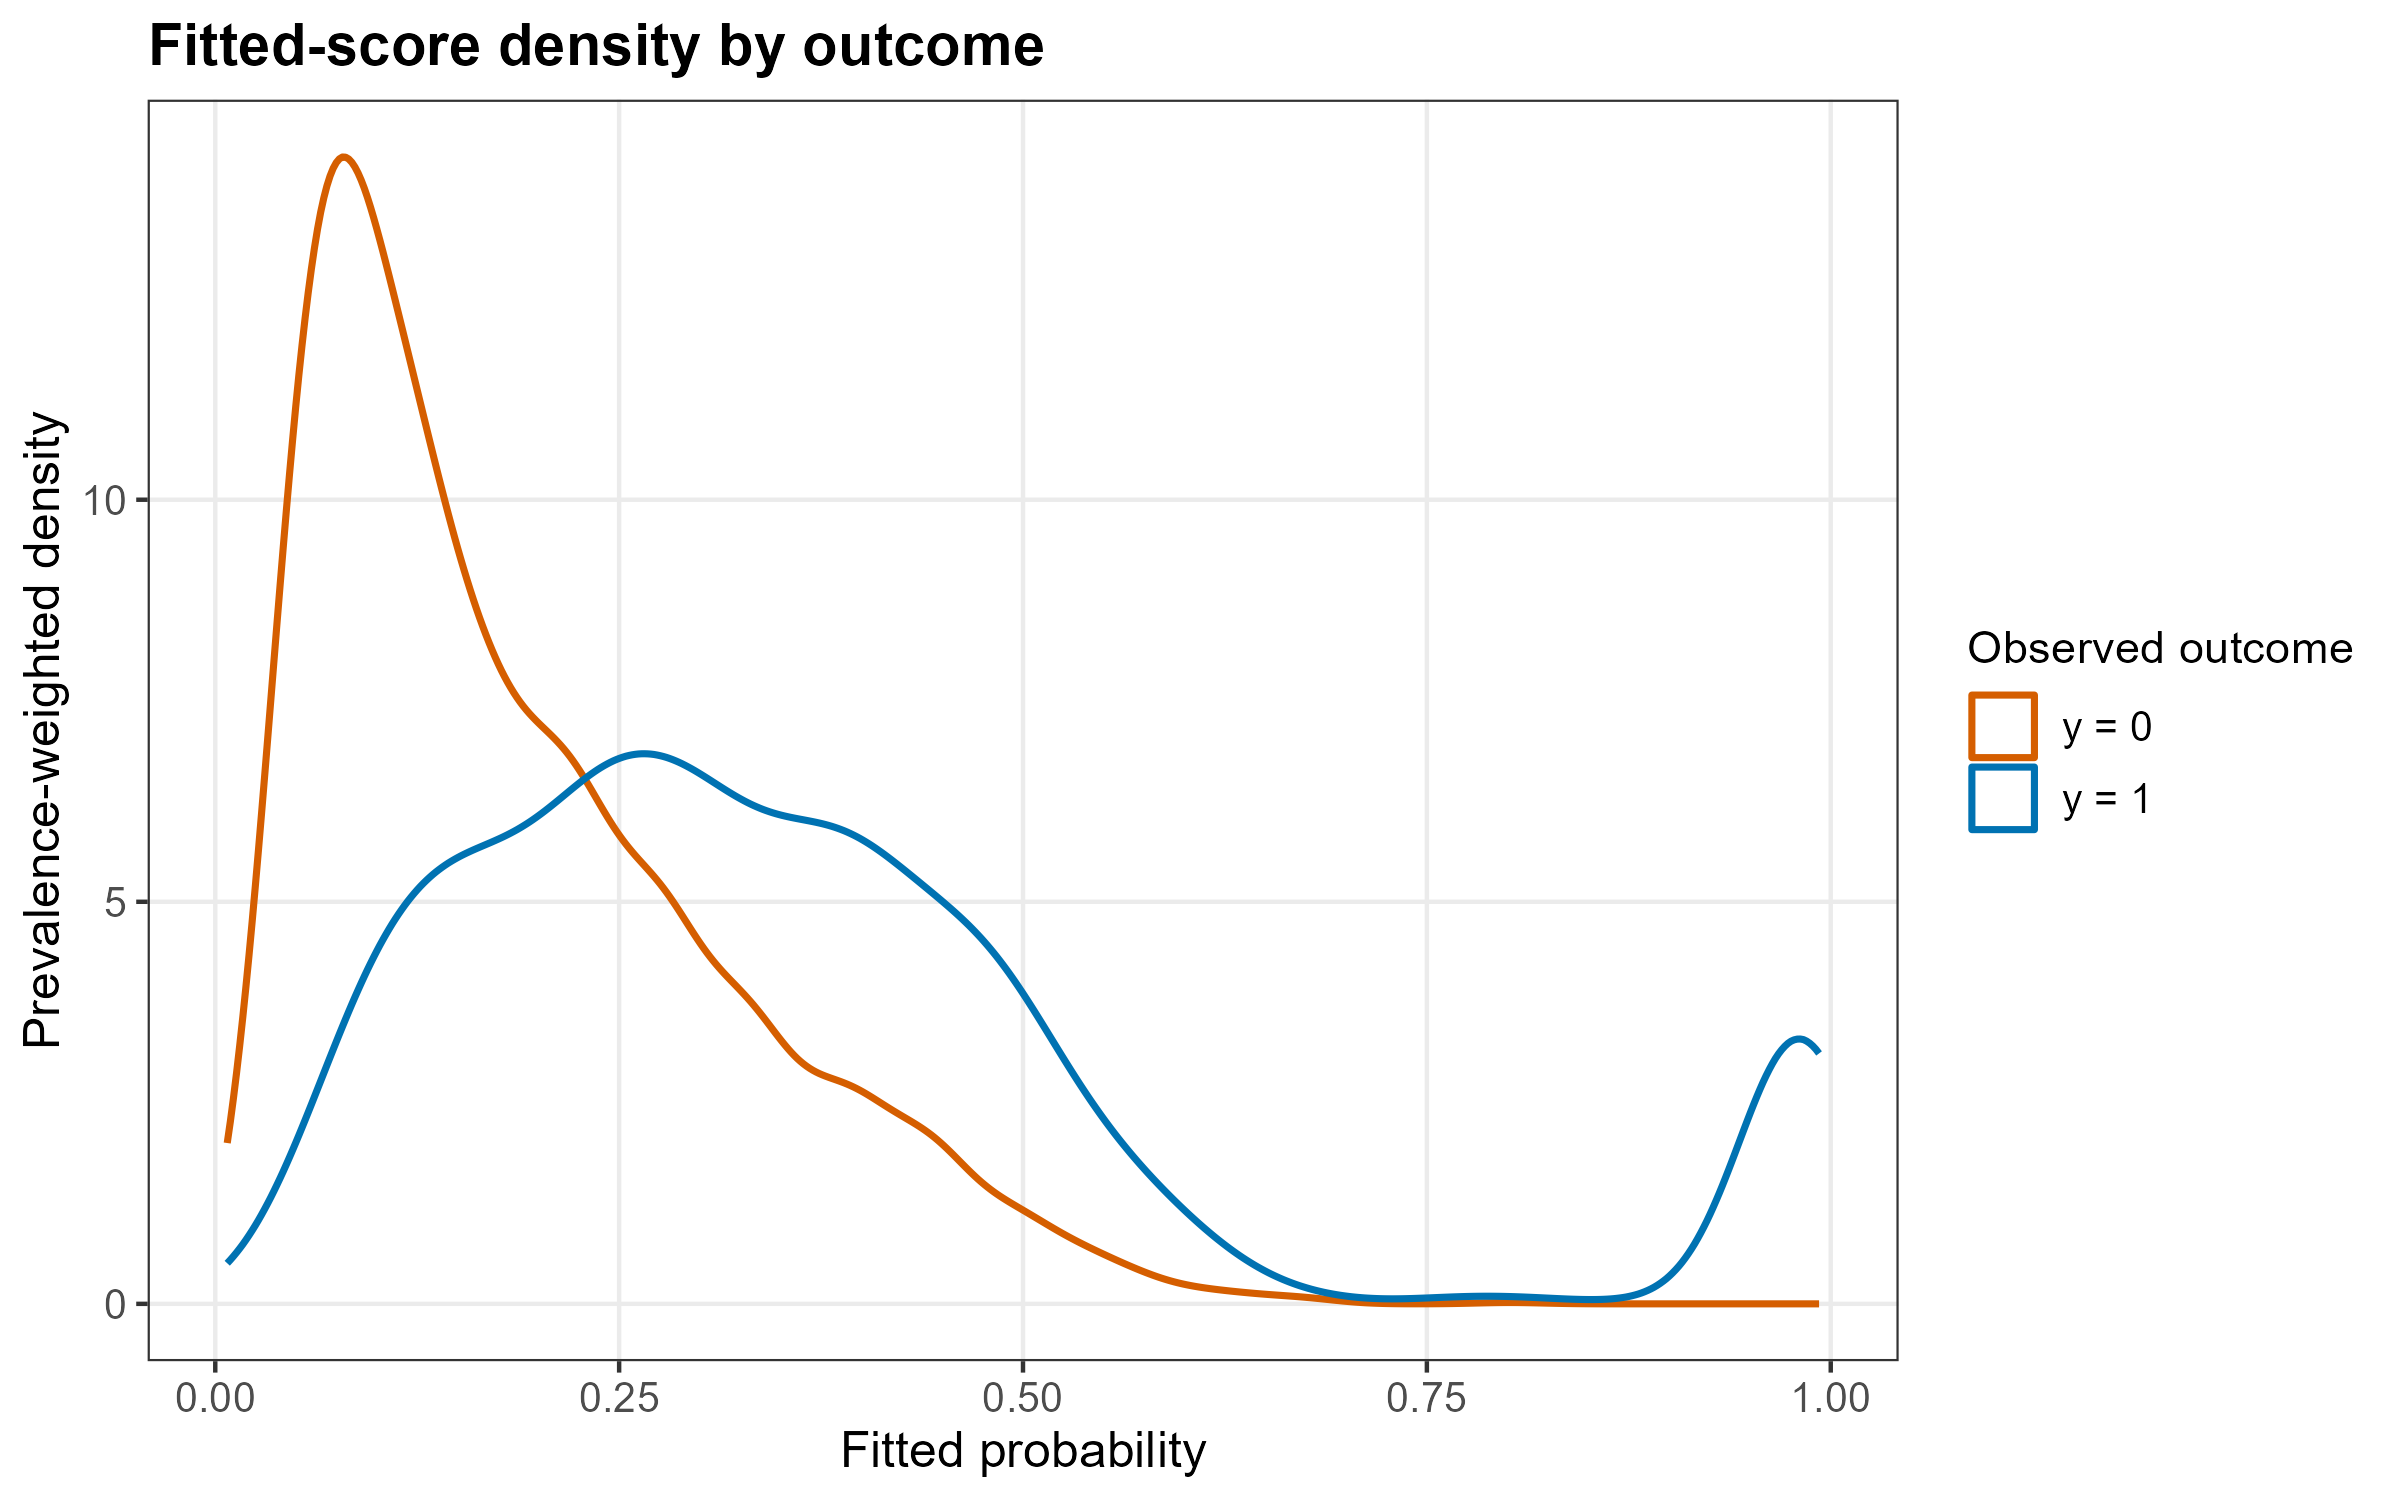
\includegraphics[width=\textwidth]{Figures/Results/real data/score_density_y_overlay.png}
        \caption{Estimated probability density from the binary BPCRR model with $K = 200$ including all individuals in the dataset. The blue line shows individuals with $y = 1$, and the red line shows individuals with $y = 0$.}
        \label{fig:pred_density}
    \end{subfigure}

    \caption[Robustness check and score density before removing island 61]{
    Robustness check and score density before removing island 61.
    }
    \label{fig:island61_and_density}
\end{figure}

%\section{Application results (Mathilde)}
%\todo[inline]{Please use a meaningful title, such as: Prediction of breeding values for disperal}
% -------------- CV on BVs for both datasets results ------------

To assess whether the breeding values estimated by the models contributed meaningfully to the prediction of dispersal, we performed 10-fold cross-validation on both datasets and evaluated the estimated breeding value against the dispersal status $0/1$ with the PR-AUC  (\autoref{fig:pr_auc_comparison}). Across all 10 folds, both the linear and the binary model performed better than a random classifier, as the PR-AUC exceeded the prevalence in the data, which was $0.09$ for the autumn dispersal dataset and $0.23$ for the adult dispersal dataset. Overall, the linear and binary models appeared to perform similarly. For the autumn dispersal dataset, the PR-AUC ranged from $0.11$ to $0.29$, corresponding to a $22\%$--$222\%$ increase in predictive performance relative to a random classifier (\autoref{fig:pr_auc_autumn}). The mean PR-AUC across all 10 folds was approximately $0.15$, corresponding to a $66\%$ increase. For the adult dispersal dataset, we observed a generally higher PR-AUC across all folds, ranging from $0.30$ to $0.39$, which corresponds to a relative increase in predictive performance of $30\%$ to $70\%$ compared with a random classifier (\autoref{fig:pr_auc_comparison}). The overall mean PR-AUC across the 10 folds was $0.34$, corresponding to a $48\%$ relative increase.  

% ------------- CV on BVs for both datasets ----------------

\begin{figure}[htbp]
      \centering
      \begin{subfigure}[t]{0.48\textwidth}
          \centering
          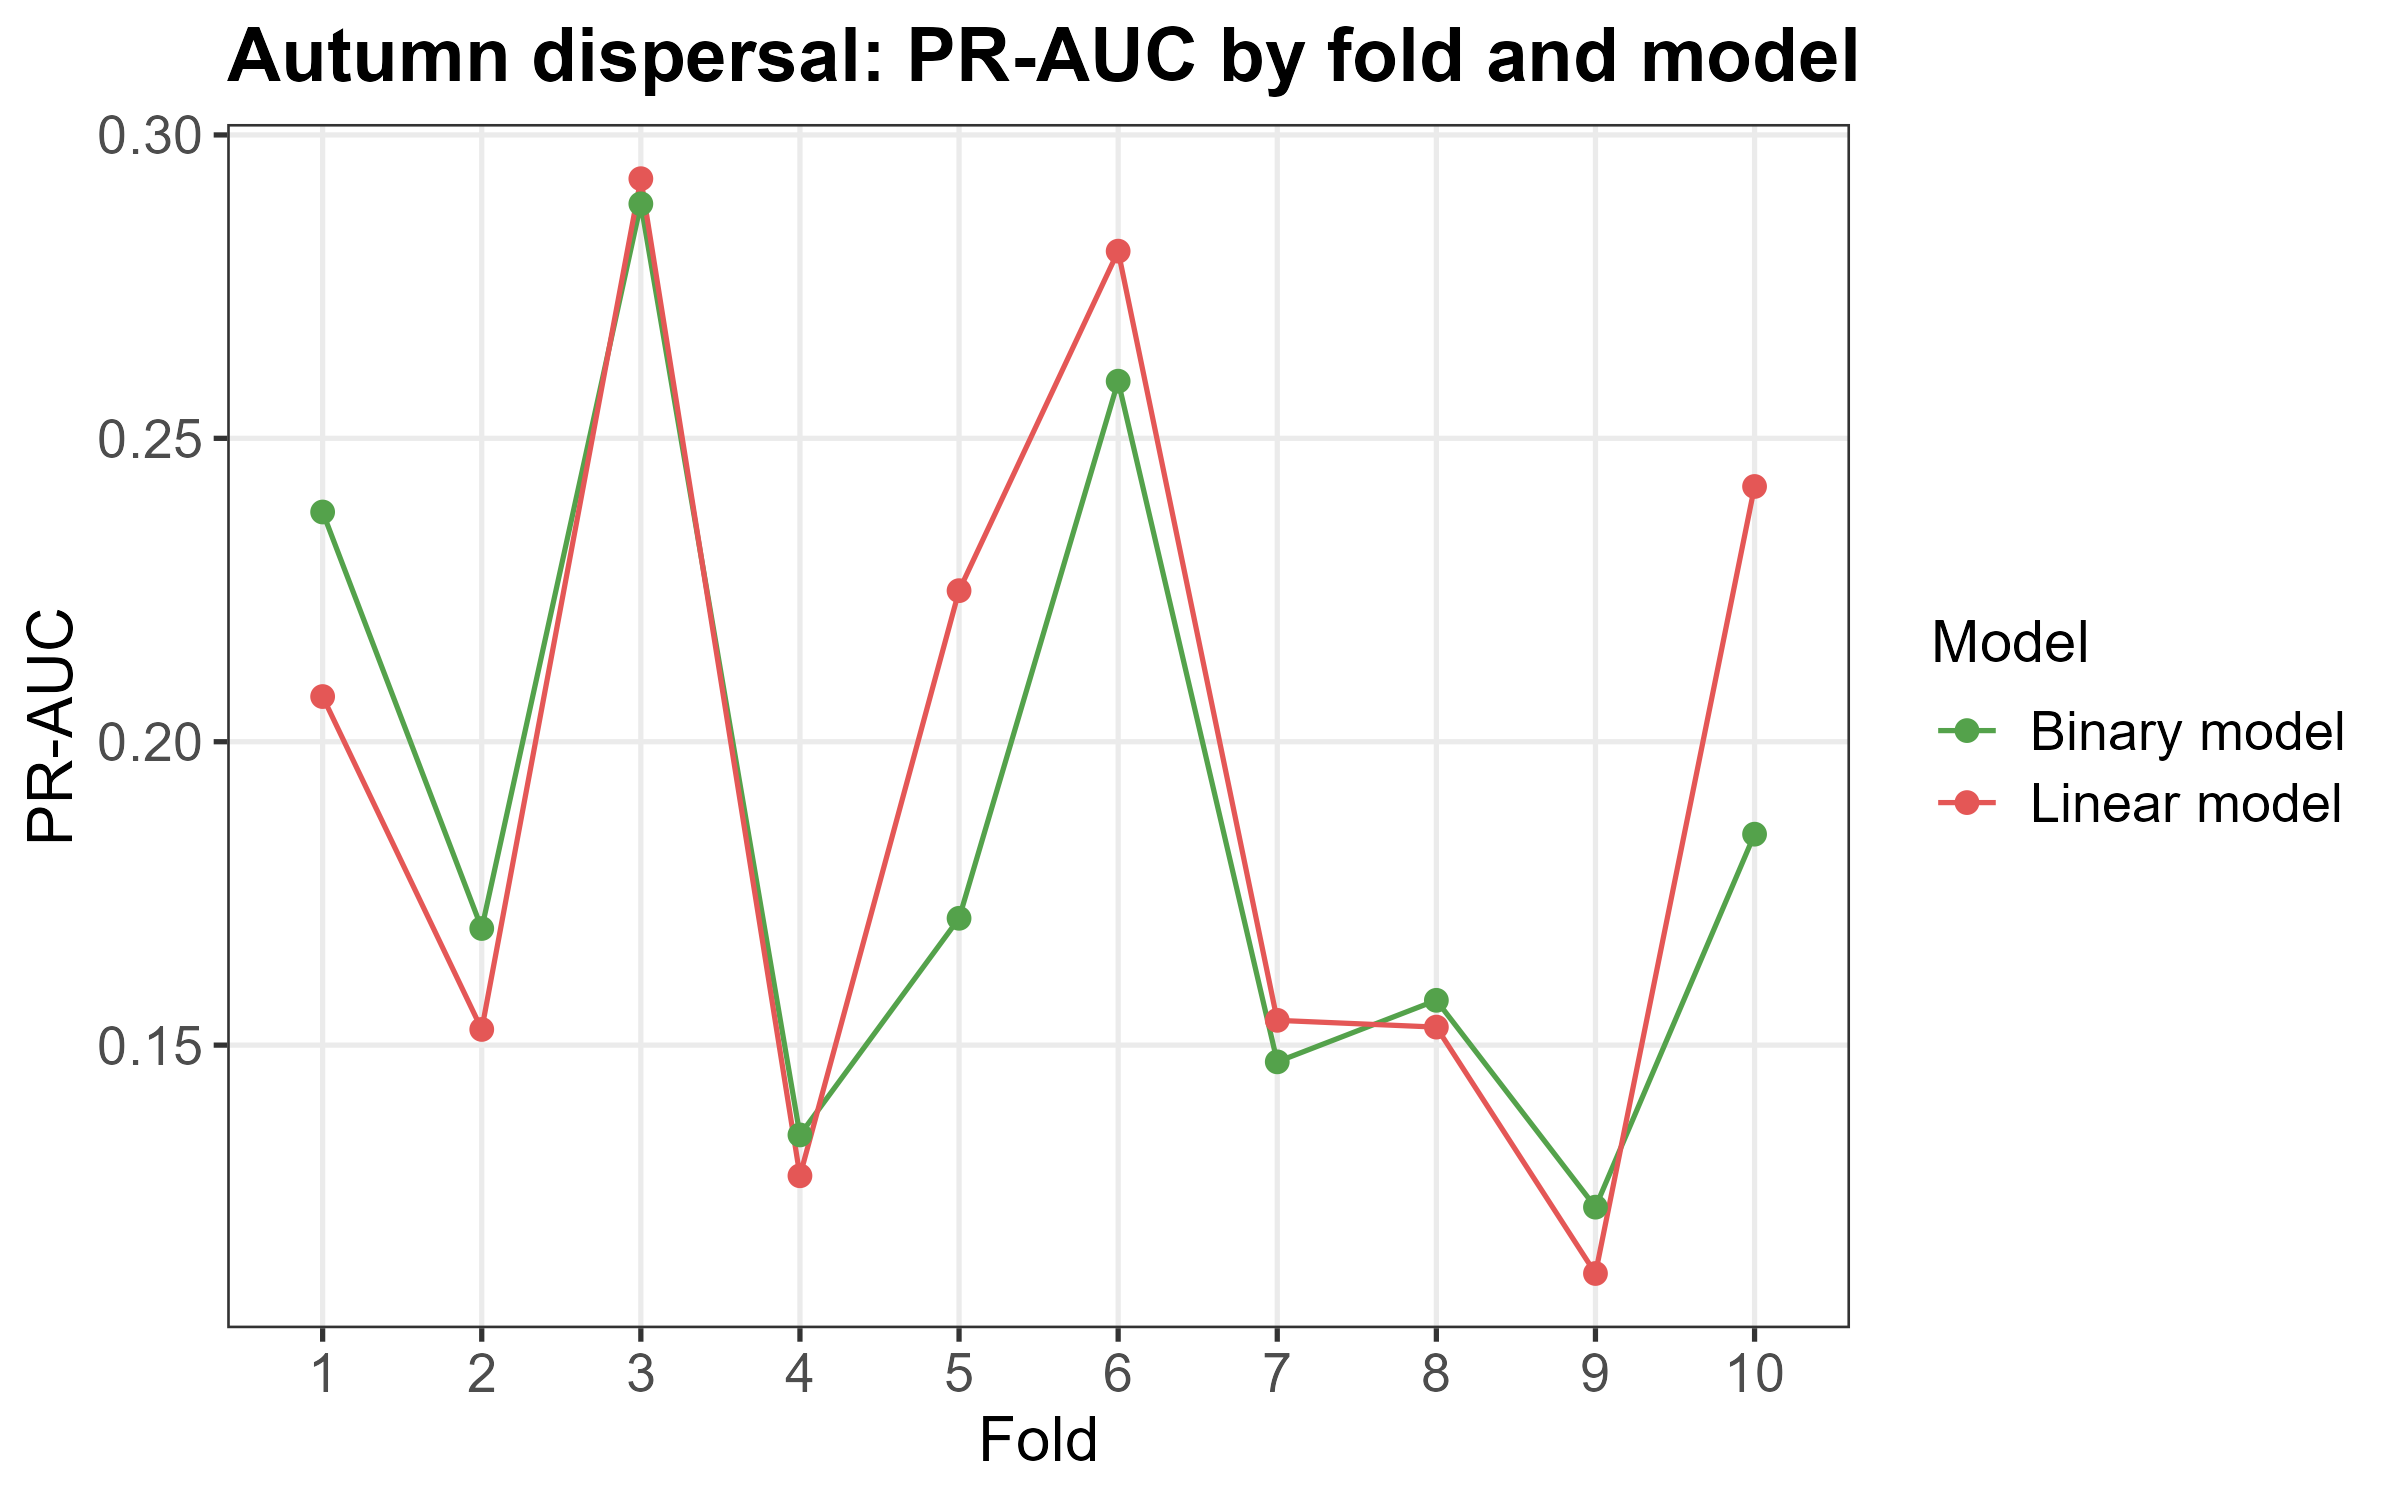
\includegraphics[width=\linewidth]{Figures/Results/application_results/autumn_dispersal_bin_vs_lin_fold_pr_auc.png}
          %\caption{Autumn dispersal data.}
          \label{fig:pr_auc_autumn}
      \end{subfigure}
      \hfill
      \begin{subfigure}[t]{0.48\textwidth}
          \centering
          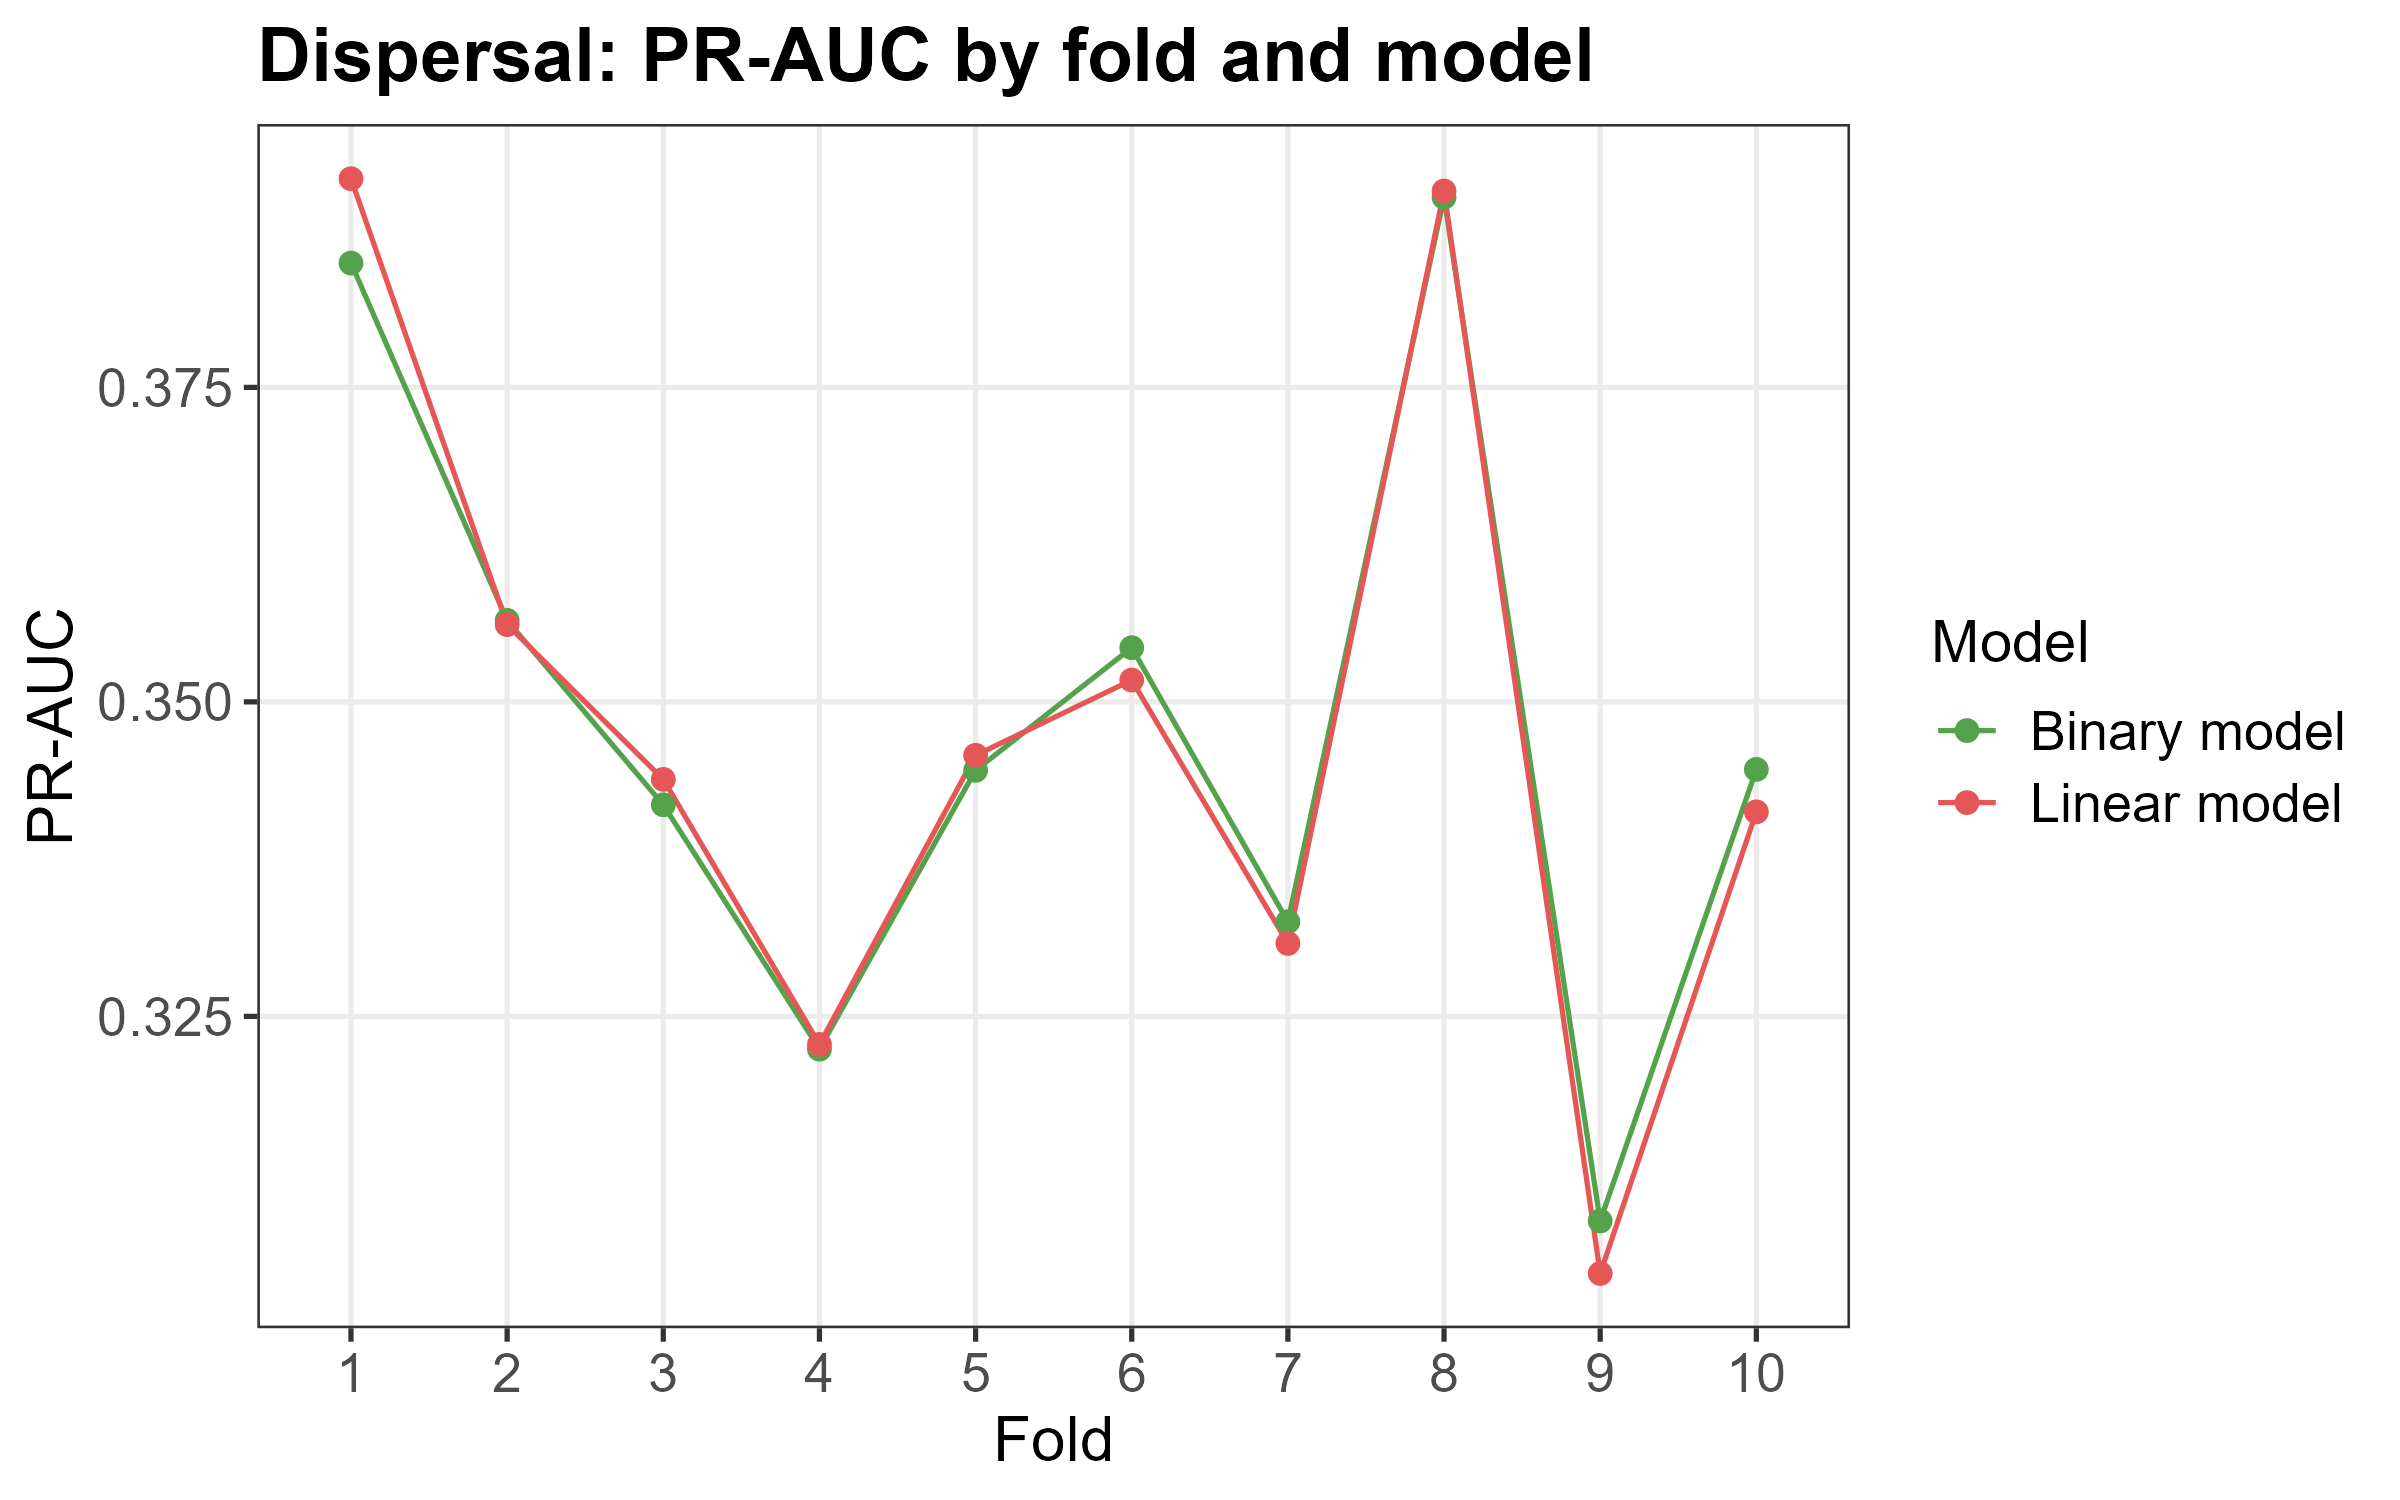
\includegraphics[width=\linewidth]{Figures/Results/application_results/big_dataset_bin_vs_lin_fold_pr_auc.png}
          %\caption{Adult dispersal data. }
          \label{fig:pr_auc_mathilde}
      \end{subfigure}
      \caption{Fold-wise PR-AUC for the binary and linear models across the autumn dispersal data (left) and the dispersal data (right).}
      \label{fig:pr_auc_comparison}
  \end{figure}